%%    _____  _____
%%   |  __ \|  __ \    AUTHOR: Pedro Rivero
%%   | |__) | |__) |   ---------------------------------
%%   |  ___/|  _  /    DATE: April 28, 2020
%%   | |    | | \ \    ---------------------------------
%%   |_|    |_|  \_\   https://github.com/pedrorrivero
%%

% \documentclass[9pt, aspectratio=169]{beamer}
\documentclass[9pt, handout, aspectratio=169]{beamer}	% Skip \pause commands
\usetheme{PRRwide}
\usepackage{PRRmath}

% \setbeameroption{show notes}
% \setbeameroption{show only notes}

%% ----------------------------------------------------------------------------
%% FRONT-MATTER
%% ----------------------------------------------------------------------------

\title{Quantum Computation for the Understanding of Mass}
\subtitle{Simulating Quantum Field Theories}
\author{Pedro Rivero}
\institute{Illinois Institute of Technology \\ Argonne National Laboratory}
\newcommand{\mail}{priveroramirez@hawk.iit.edu}
\date{\today}
\newcommand{\website}{
	\href{https://www.iit.edu/physics}
	{www.iit.edu/physics}
}

\begin{document}
	\justify
	\setlength{\abovedisplayskip}{0pt}
	\setlength{\belowdisplayskip}{12pt}
	\setlength{\abovedisplayshortskip}{0pt}
	\setlength{\belowdisplayshortskip}{12pt}

\begin{frame}[plain,t]
	\titlepage
\end{frame}

% \begin{frame}[c]{Contents}
% %		\begin{multicols}{2}
% %  			\tableofcontents
% %		\end{multicols}
% 	\tableofcontents
% \end{frame}


%% ----------------------------------------------------------------------------
%% MAIN-MATTER
%% ----------------------------------------------------------------------------

\section{Introduction}

\begin{frame}{Introduction}

	Nature is described through the mathematical framework provided by \textbf{Quantum Field Theory}.

	\begin{multicols}{2}

		\begin{itemize}
			\item<2-> The different implementations of Quantum Field Theory are referred to as quantum field theories themselves.
			\item<3-> Quantum Chromodynamics (QCD) is the theory of the strong nuclear force.
			\item<3-> QCD holds many mysteries (e.g. \textbf{mass generation} phenomena).
			\item<4-> QCD is currently studied using brute-force numerics on the world’s largest supercomputers.
			\item<4-> Many aspects of quantum field theories cannot be studied using classical computers.
		\end{itemize}

		\begin{center}
			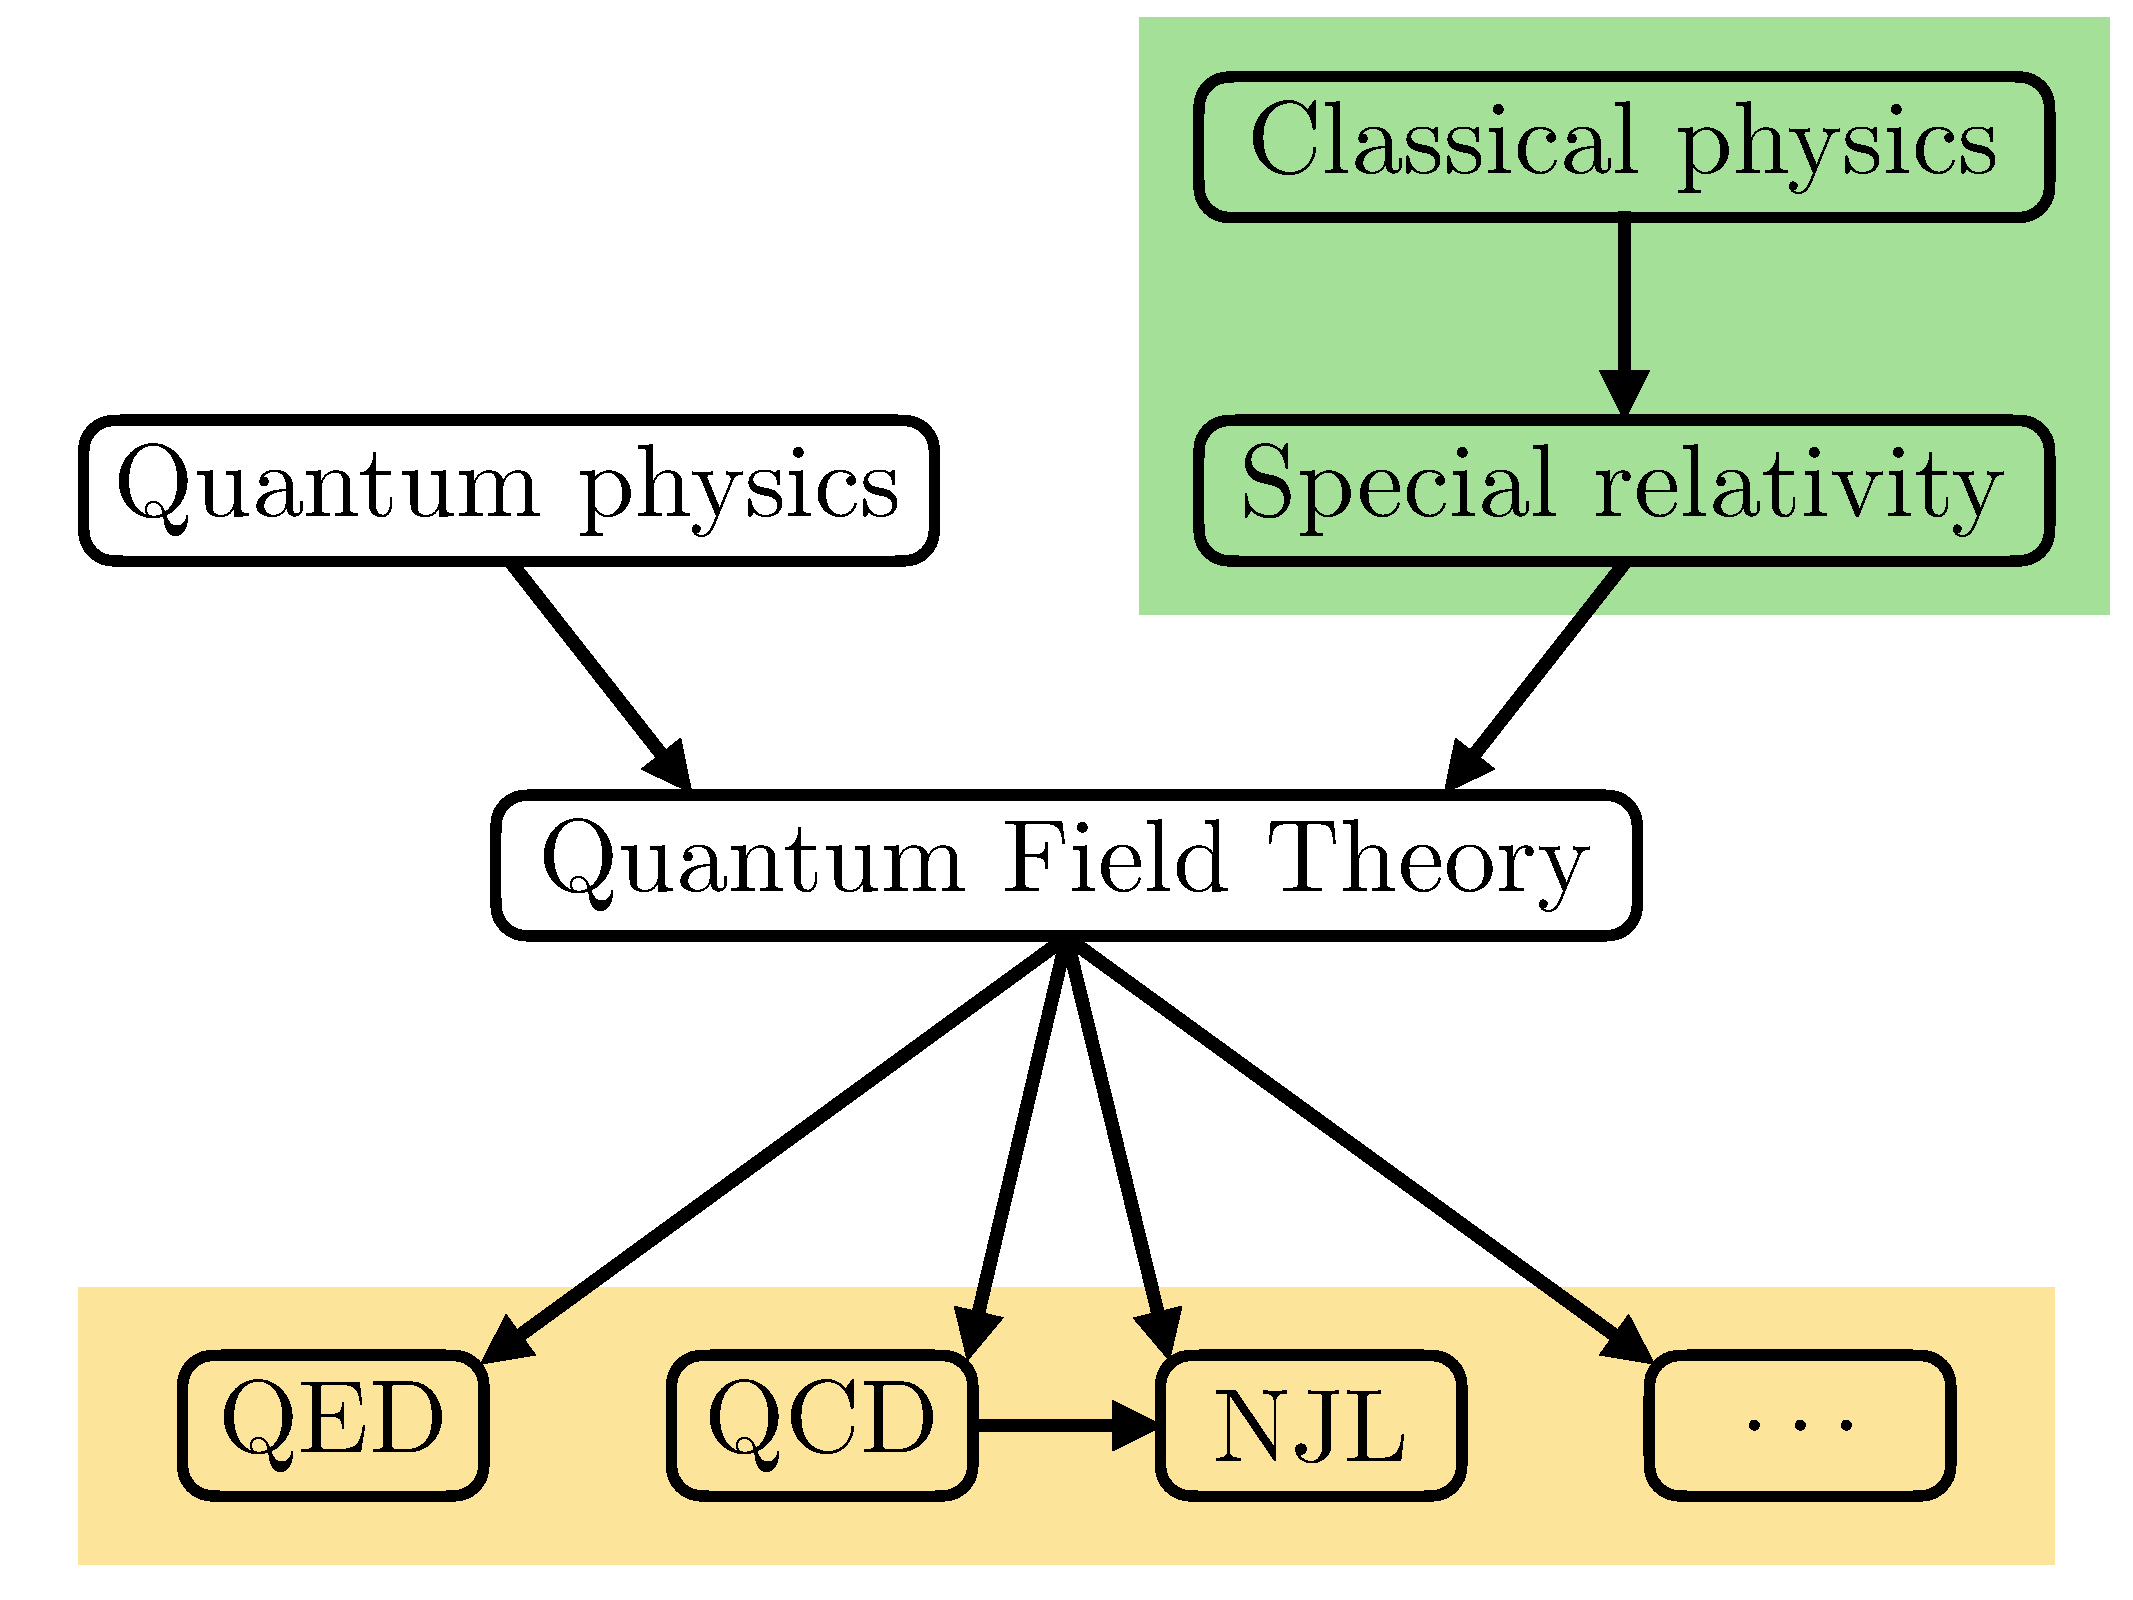
\includegraphics[width=.40\paperwidth]{Figures/quantum-field-theory}
		\end{center}

	\end{multicols}

\end{frame}

%% ----------------------------------------------------------------------------

\begin{frame}{Objectives}

	An important path forward is to develop methods to simulate these models on quantum computers. This effort is only just beginning, however, performing calculations on a quantum computer is far from being a straightforward task; and it has only been achieved for relatively simple problems. My goal will be to develop some of the techniques necessary to use quantum computers for this endeavor. We will do so by analyzing the following:

	\medskip

	\begin{itemize}
		\item<2-> \textbf{Nambu--Jona-Lasino model} (NJL) in $1+1$ dimensions: an effective field theory, regarded as a low-energy approximation to QCD.
		\item<3-> It retains certain key features of QCD, such as the so called Goldstone modes and \textbf{dynamical chiral symmetry breaking}; which in turn is responsible for the creation of dressed mass.
		\item<4-> This model can be solved nonperturbatively through the standard leading order truncation; an important characteristic since verifying the solutions returned by any quantum computation is currently a major challenge.
	\end{itemize}

\end{frame}

%% ----------------------------------------------------------------------------

\begin{frame}[c]{Contents}
%		\begin{multicols}{2}
%  			\tableofcontents
%		\end{multicols}
	\tableofcontents
\end{frame}

%% ----------------------------------------------------------------------------
%% ----------------------------------------------------------------------------

\section{Background in Quantum Computation}

\begin{frame}{Background in Quantum Computation}

	Before the abacus was invented, the only way of counting was through a "thermometer-like" scale. This device introduced the concept of \textbf{digits}, which was later adopted into our own language in the form of \textbf{numerals}. This meant that, instead of counting up to $N$ using $N$ elements, we could count using only $\text{log}_b (N)$ abacus elements ---where $b$ is the base of our number system (i.e. the amount of beads per row in the abacus).

		\begin{multicols}{2}

		 	Therefore, for $b\geq2$, the abacus introduced an \textbf{exponential decrease in resource requirements}.

			\medskip

			Quantum computers do something analogous. To represent the quantum state of a system made out of $N$ subsystems ---with $b$ degrees of freedom each--- we would usually need $b^N$ classical elements (i.e. numbers). By using quantum systems for this representation, we would only need $N$ quantum elements (i.e. each subsystem).

			\columnbreak

			\begin{center}
				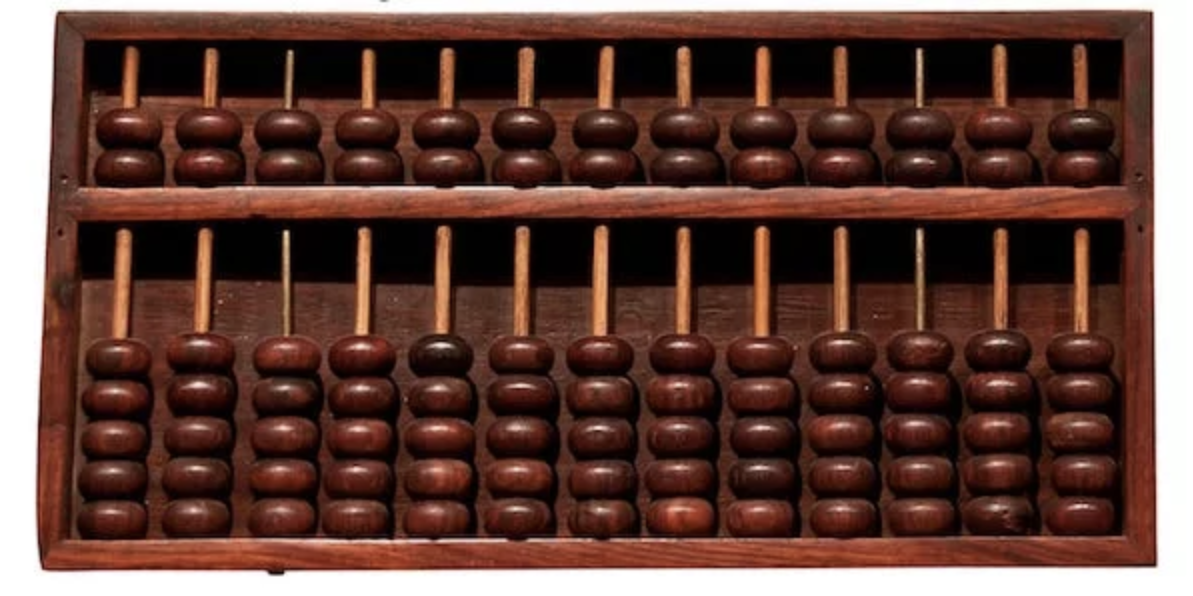
\includegraphics[width=.30\paperwidth]{Figures/abacus} \\
				\vspace{10pt}
				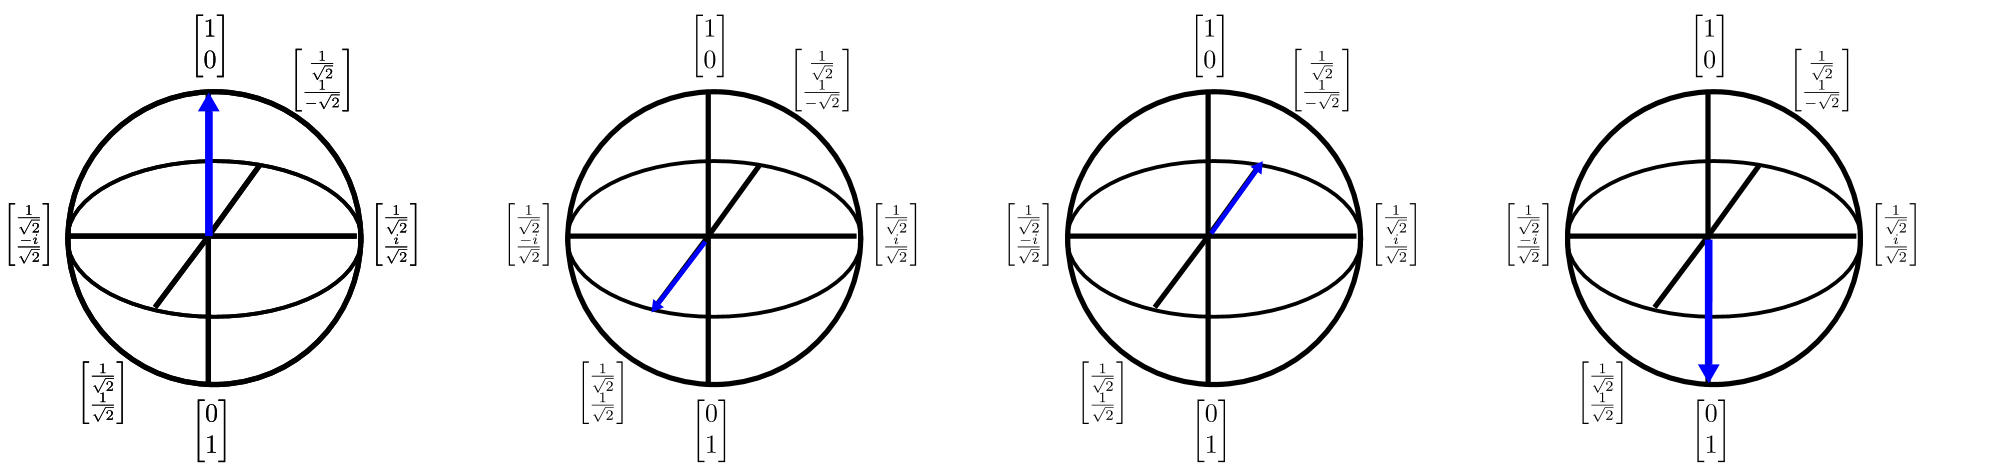
\includegraphics[width=.34\paperwidth]{Figures/qubits}
			\end{center}

		\end{multicols}

\end{frame}

%% ----------------------------------------------------------------------------

\subsection{Quantum logic}

\begin{frame}{Quantum logic}

	Formally speaking, the states of a quantum system will be represented as a vector in a Hilbert space; whereas the state of a classical system is simply an element of a set. This distinction, along with the probabilistic nature of quantum mechanics, makes the entire logical system describing quantum computers fundamentally different than \textbf{classical propositional logic} (i.e. Boolean algebra).

	% Because these logical systems are so different from each other, if we are to take advantage of the power of quantum mechanics for performing computations, it is essential to “think” in quantum terms; and formulate the problems that we want to solve according to this new logic.

	\begin{multicols}{2}

		\action<2->{
			\underline{\textbf{CLASSICAL LOGIC}}\\
			\small{\emph{Set Theory (Boolean algebra)}}

			\medskip

			\begin{itemize}
				\item \textbf{AND} $\quad \Rightarrow \quad A \cup B$
				\item \textbf{OR} $\quad \Rightarrow \quad A \cap B$
				\item \textbf{NOT} $\quad \Rightarrow \quad \overline{A}$
				\item \textbf{XOR} $ \quad \Rightarrow \quad A \cap B - A \cup B$
			\end{itemize}
		}

		\columnbreak

		\action<3->{
			\underline{\textbf{QUANTUM LOGIC}}\\
			\small{\emph{Quantum Theory (Non-abelian)}}

			\medskip

			\begin{itemize}
				\item \textbf{Probabilistic measurement}
				\item \textbf{Measurement causes disturbance}
				\item \textbf{Superposition}
				\item \textbf{Entanglement}
				\item \textbf{Uncertainty principle}
			\end{itemize}
		}

	\end{multicols}

\end{frame}

%% ----------------------------------------------------------------------------

\subsection{Quantum information}

\begin{frame}{Qubits and the Bloch sphere}

	\begin{multicols}{2}

		The basic unit of information in quantum mechanics is the \textbf{qubit}; a quantum system with only two distinguishable states: $\ket{0}$ and $\ket{1}$.

		\medskip

		The main difference between bit and qubit lays in the fact that, when they are not being measured, quantum systems do not need to be in one of their so called, mutually incompatible, basis states; instead, they can be in any (normalized) \textbf{linear superposition} of them.

		\medskip

		A simple example of a qubit is a spin-$\frac{1}{2}$ particle; whose space of states is spanned by the spin up and spin down quantum basis. Inspired by this particular system, the qubit can be pictorially represented through the \textbf{Bloch sphere}.

		% This allows us to visualize non-commutative quantum logic.

		\columnbreak

		\begin{center}
			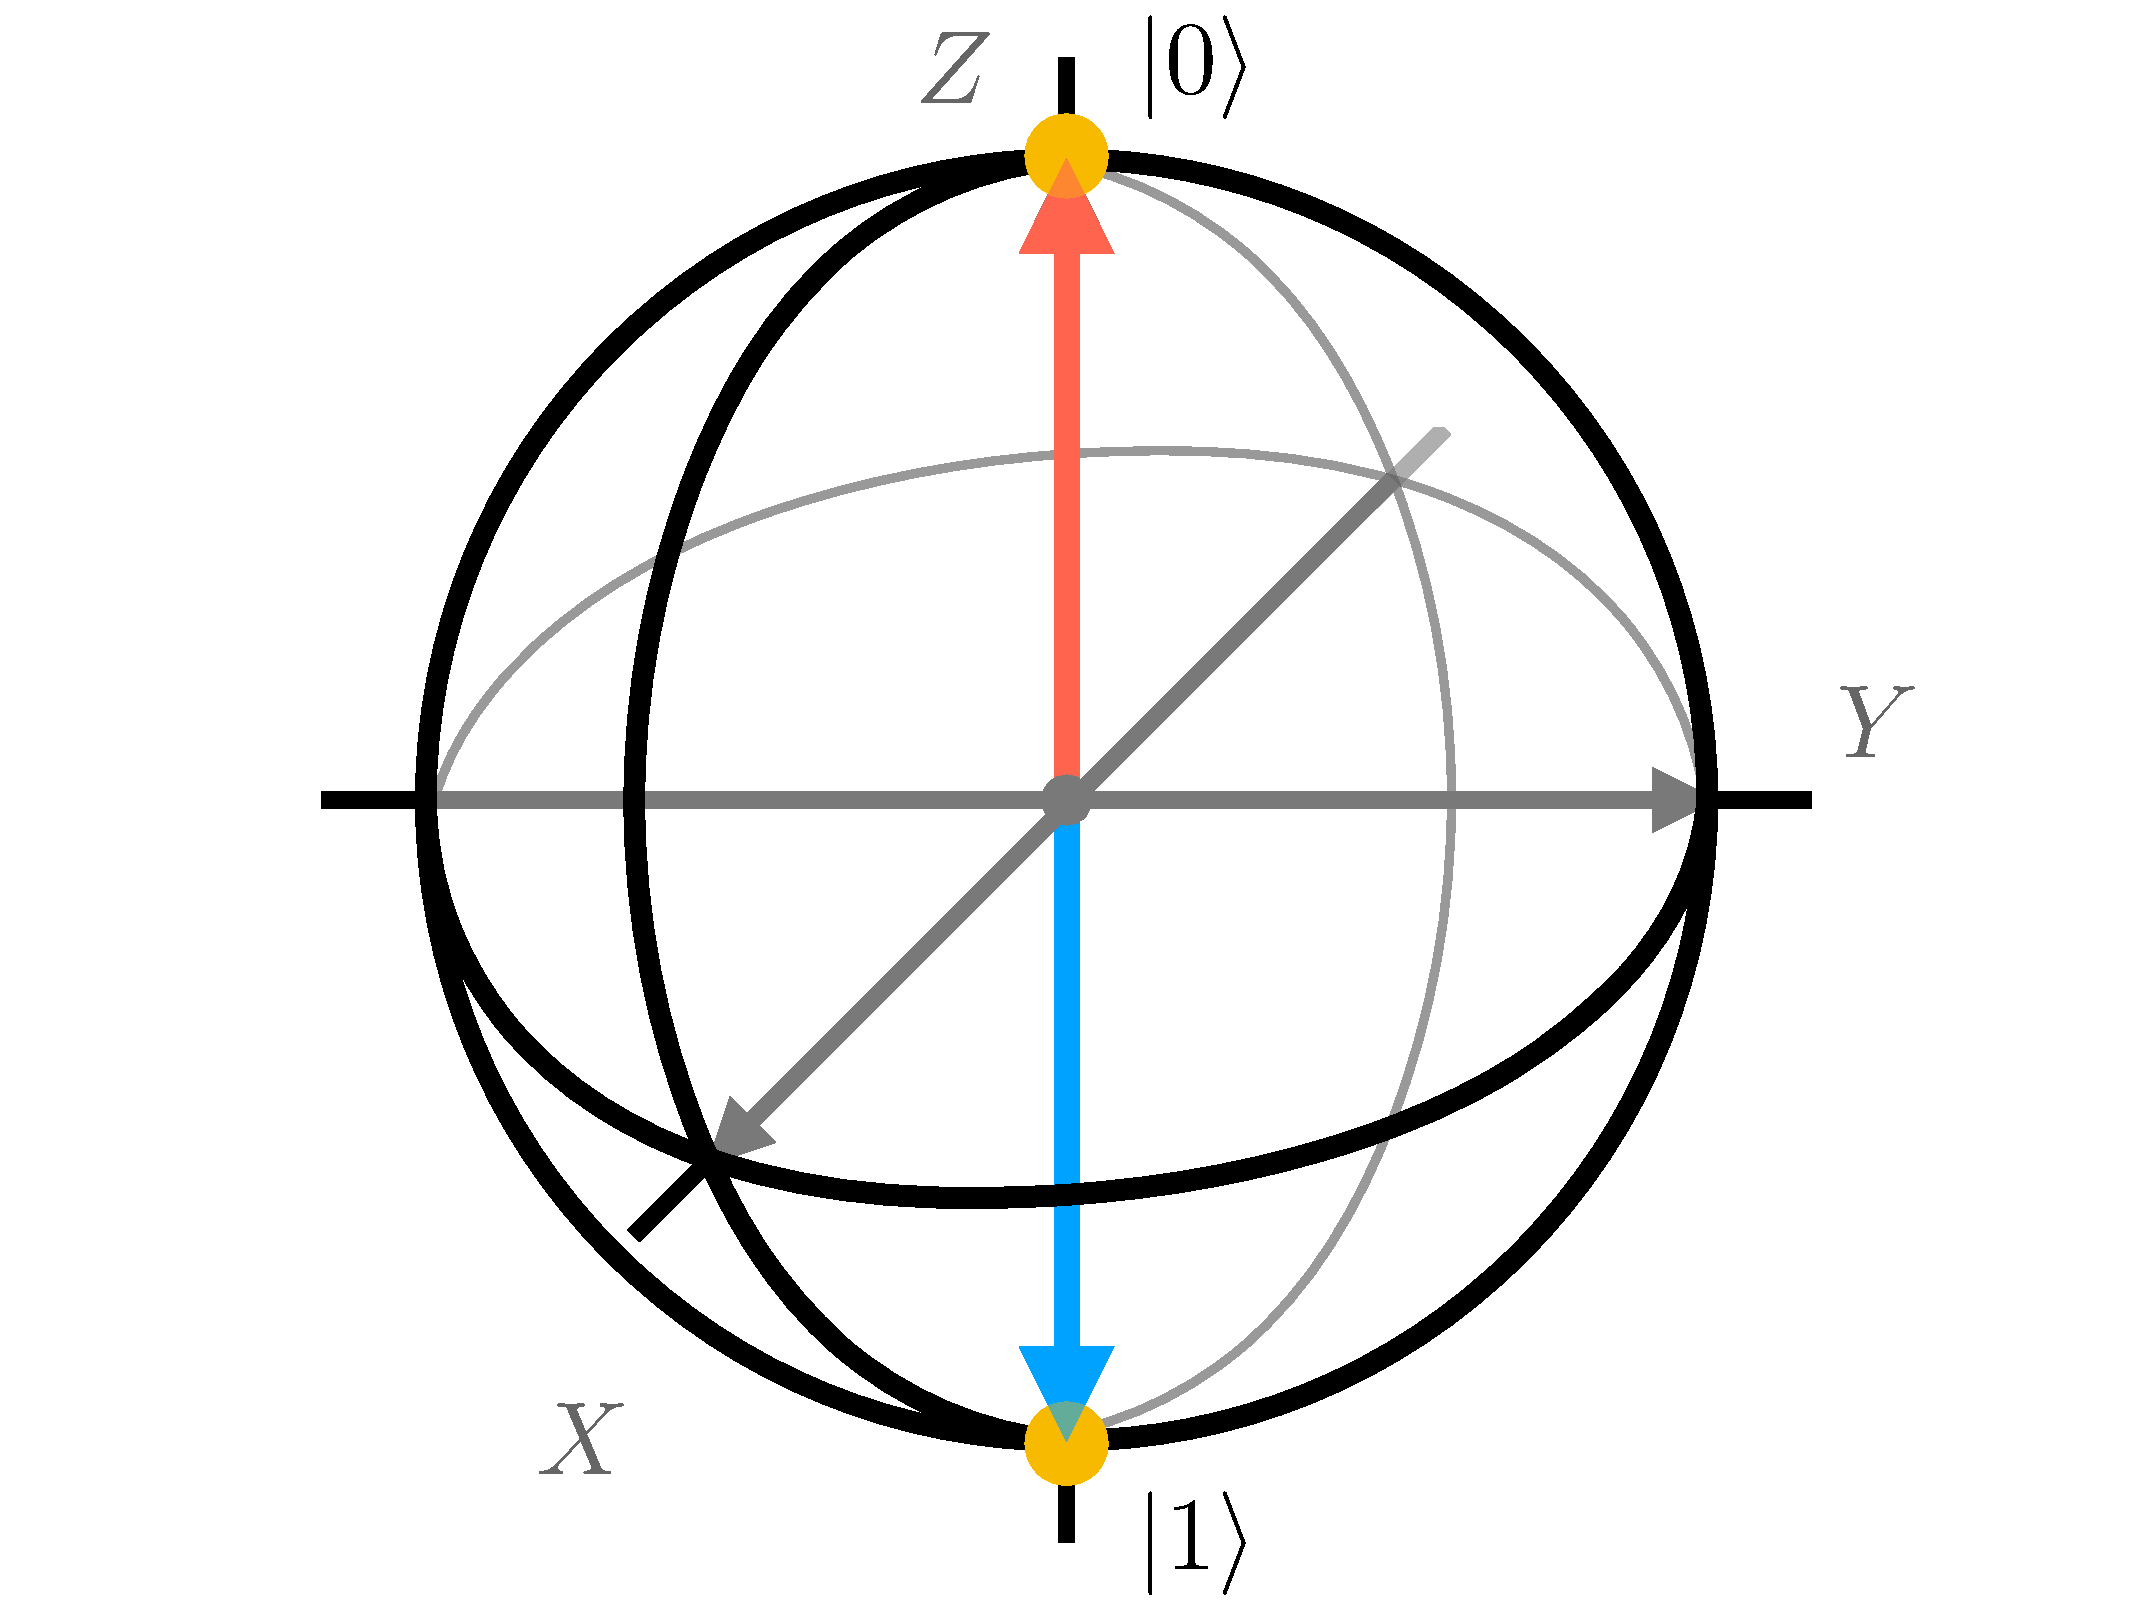
\includegraphics[width=.40\paperwidth]{Figures/quantum-background/bloch-sphere}
		\end{center}

	\end{multicols}

\end{frame}

%% ----------------------------------------------------------------------------

\begin{frame}{Quantum information}

	In the same way that the device known as an abacus had its theoretical counterpart in positional number systems, quantum computers have Quantum Information Science (QIS); which help us understand the full capabilities of these new machines. Two very important insights extracted from QIS, and with direct applicability to quantum apparatuses are:

	\medskip

	\begin{itemize}
		\item<2-> \textbf{Unitary quantum state transformations} (i.e. reversible):\\
			\begin{gather*}
			  \braket{\psi_0}{\phi_0} \equiv \braket{\psi(t)}{\phi(t)} =
					\mel{\psi_0}{U^\dagger U}{\phi_0} \qRa U^\dagger U \equiv \mathds{1}
			\end{gather*}
		\item<3-> \textbf{No-cloning theorem}:\\
			\begin{gather*}
			  U_\text{cloning} \qty(\ket{\psi}_A \otimes \ket{e}_B) =
			    \ket{\psi}_A \otimes \ket{\psi}_B \qc
				U_\text{cloning} \qty(\ket{\phi}_A \otimes \ket{e}_B) =
			    \ket{\phi}_A \otimes \ket{\phi}_B \\
			\end{gather*}
			\vspace{-3em}
			\begin{align*}
				\braket{\psi}{\phi} &=
					\qty(\braket{\psi}{\phi})_A \qty(\braket{e}{e})_B =
					\qty(\bra{\psi}_A\otimes\bra{e}_B) \qty(\ket{\phi}_A\otimes\ket{e}_B) \\
				&\equiv \qty(\bra{\psi}_A\otimes\bra{e}_B)
						U_\text{cloning}^\dagger U_\text{cloning}
						\qty(\ket{\phi}_A\otimes\ket{e}_B) =
					\qty(\bra{\psi}_A\otimes\bra{\psi}_B)
						\qty(\ket{\phi}_A\otimes\ket{\phi}_B) \\
				&= \qty(\braket{\psi}{\phi})_A \qty(\braket{\psi}{\phi})_B =
					\qty(\braket{\psi}{\phi})^2
			\end{align*}
	\end{itemize}

\end{frame}

%% ----------------------------------------------------------------------------

\begin{frame}{Implications for quantum information technologies}

	The fact that all transformations have to preserve information (i.e. entropy), imply that they are unitary. This is the only kind of transformations that a quantum computer will be able to reproduce ideally. On the other hand, the no-cloning theorem can be used to construct inherently secure communication and data storage systems. Furthermore, it means that \textbf{superluminal communication} is impossible:

	\vspace{-2em}

	\begin{multicols}{2}

		\pause
		\begin{center}
			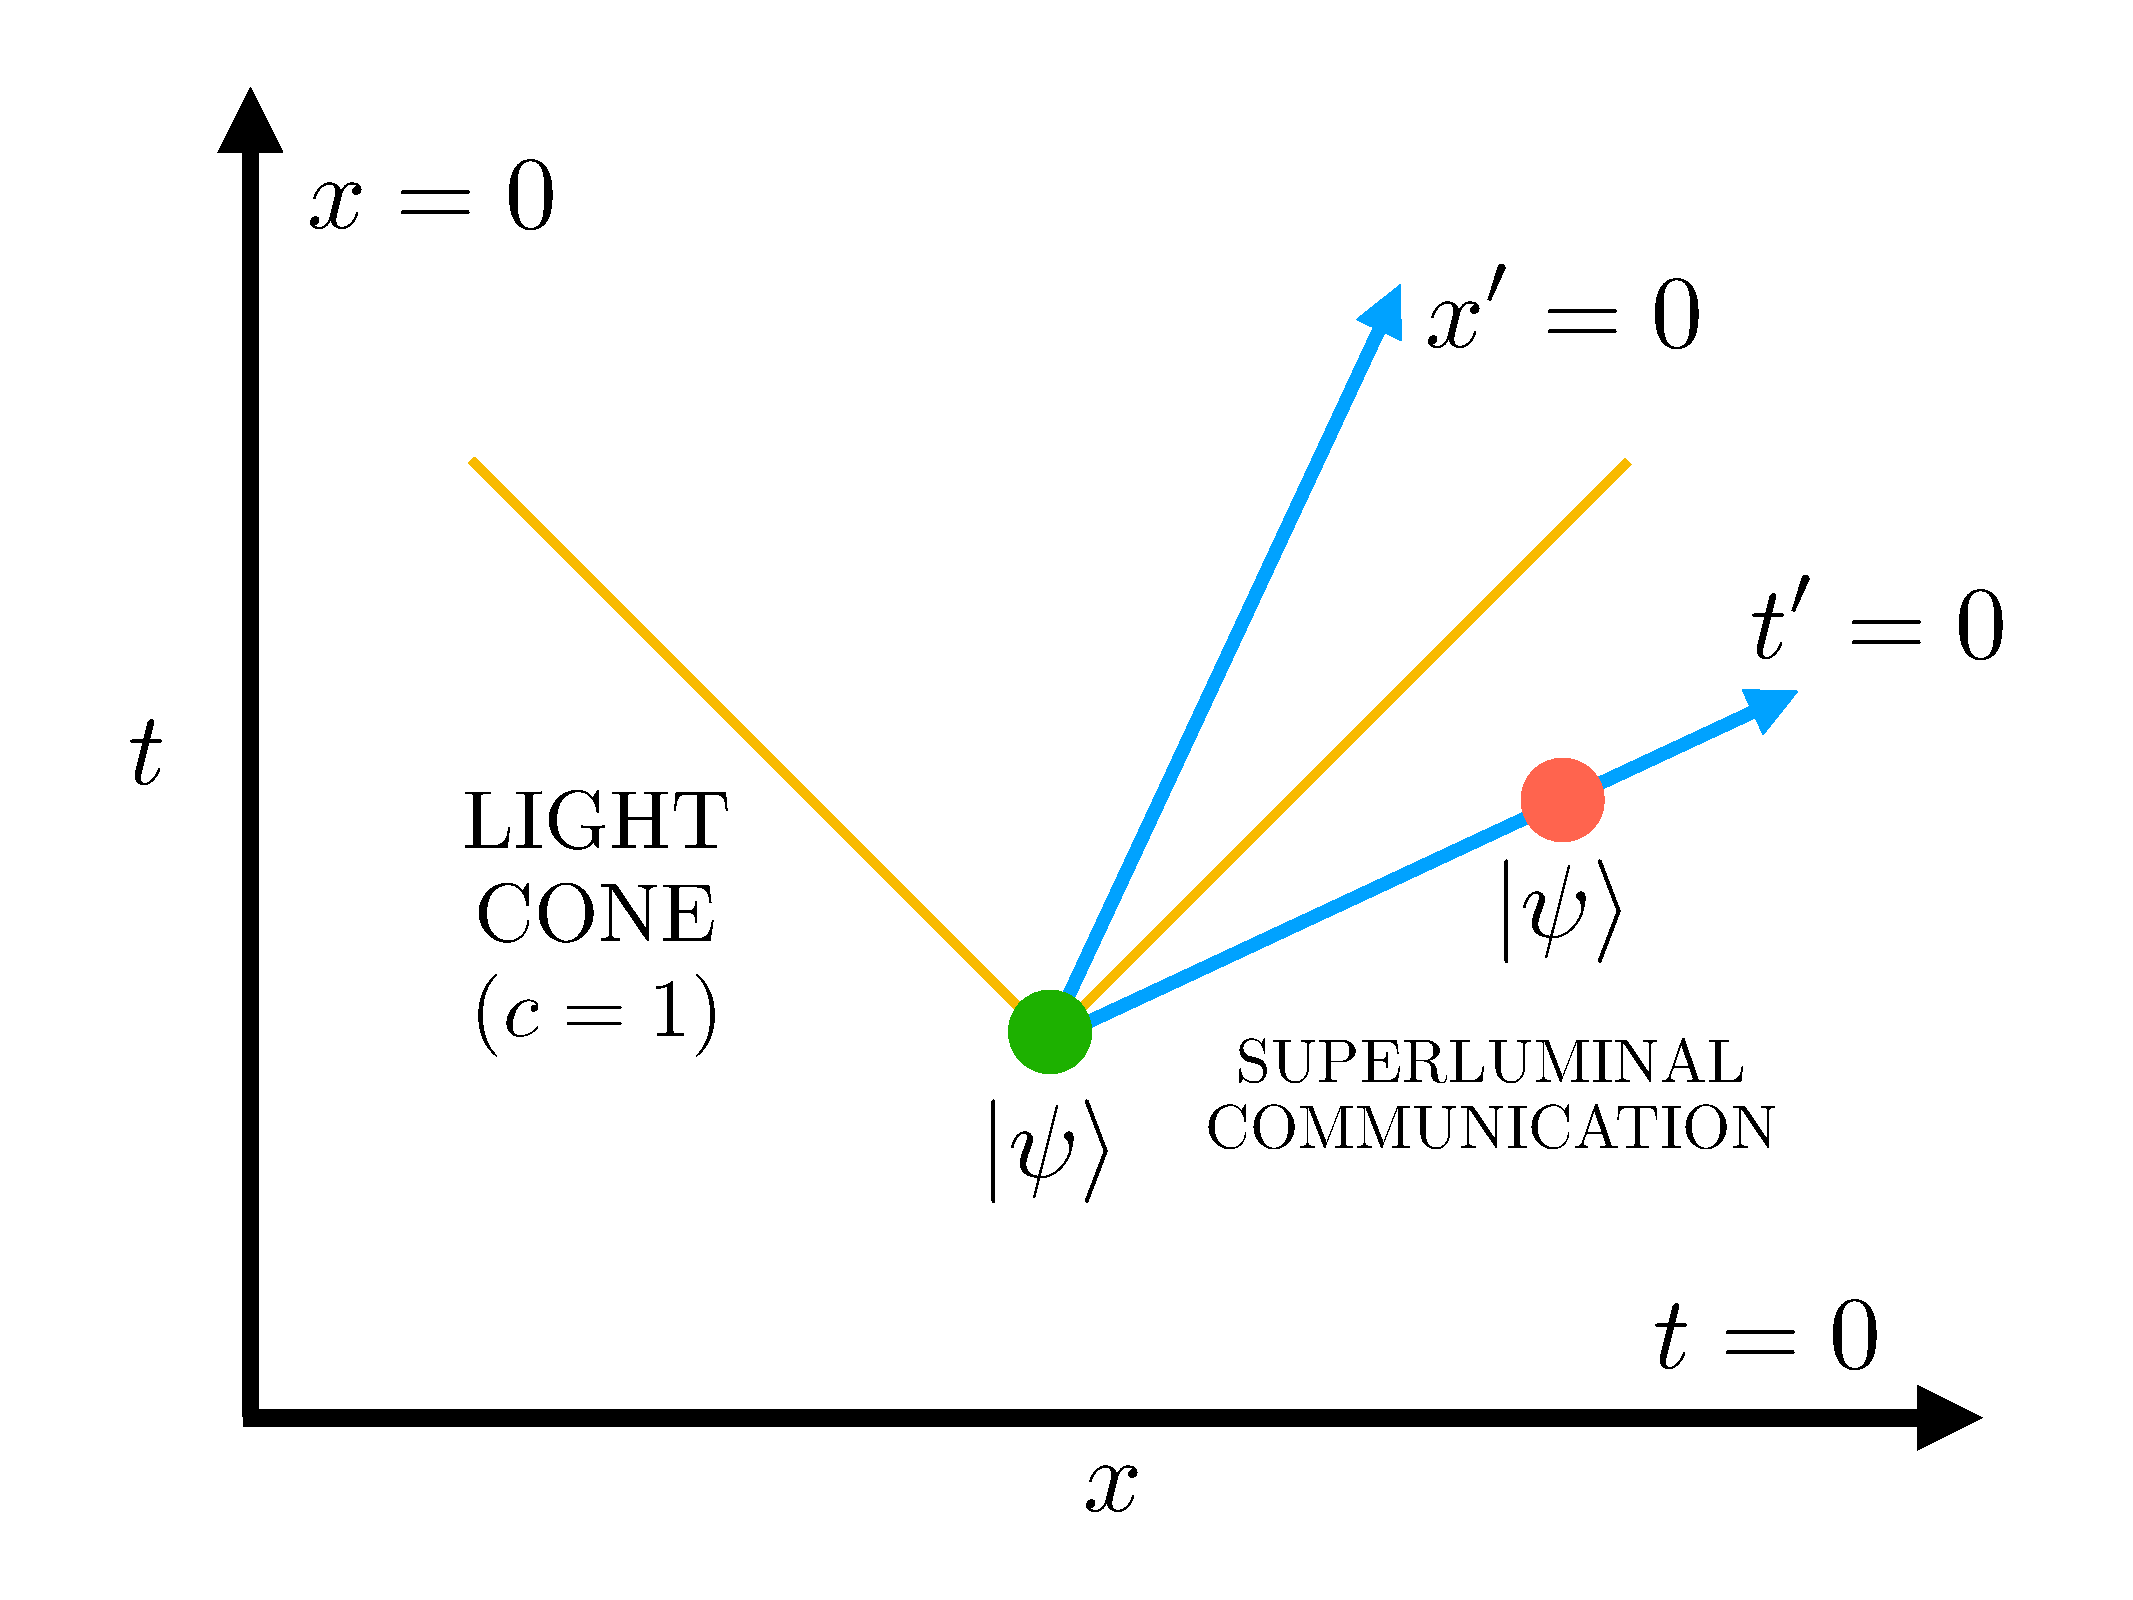
\includegraphics[width=.40\paperwidth]{Figures/quantum-background/superluminal-cloning-boost}
		\end{center}

		\columnbreak

		\pause
		\begin{center}
			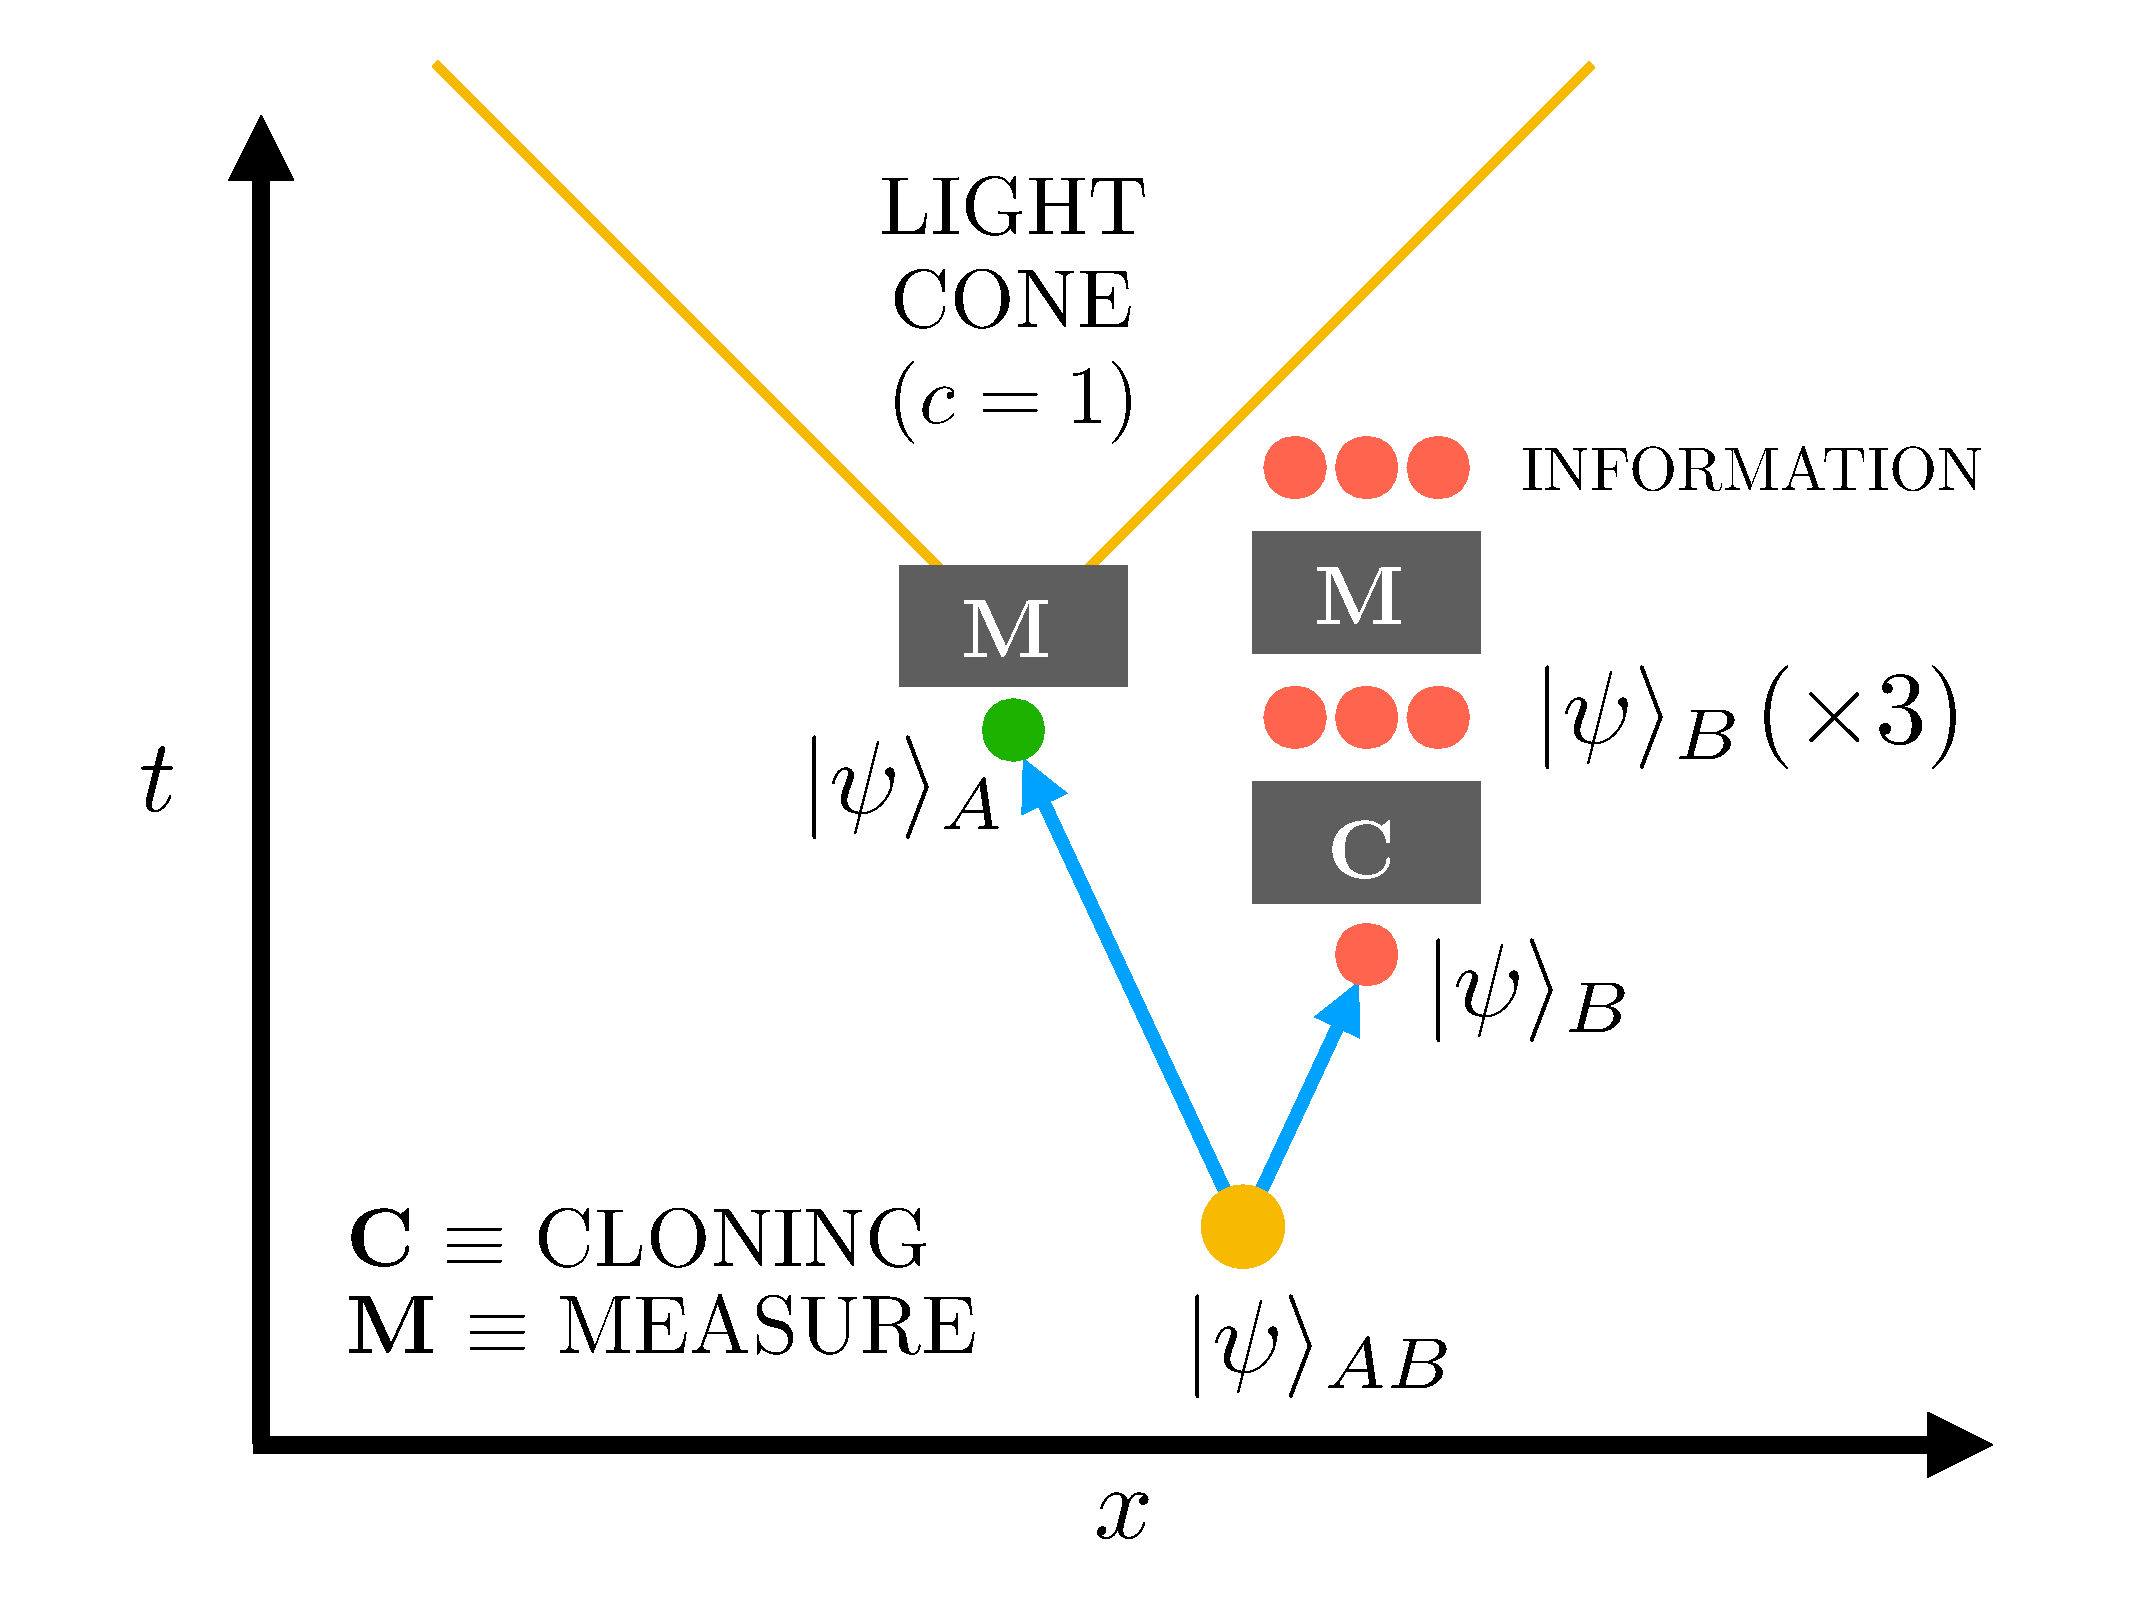
\includegraphics[width=.40\paperwidth]{Figures/quantum-background/superluminal-cloning-communication}
		\end{center}

	\end{multicols}

\end{frame}

%% ----------------------------------------------------------------------------

\subsection{Quantum computing models and algorithms}

\begin{frame}{Quantum computing models and algorithms}

	In order to work with quantum computers we need to be able to formulate how they operate in an abstract, mathematical way. There are a number of formulations that go by the name of \textbf{quantum computing models}; the main four of these being:

	\begin{multicols}{2}
		\begin{itemize}
			\item Topological
			\item Adiabatic
			\columnbreak
			\item One-way
			\item Gate arrar or circuit based
		\end{itemize}
	\end{multicols}

	\pause

	They all differ in the basic elements in which any computation is divided, and therefore have a decisive role in the \textbf{hardware implementation} of these machines. Nonetheless, all of them have been proven theoretically equivalent to each other as well as to an universal quantum Turing machine.

	\begin{multicols}{2}
		\begin{itemize}
			\item Josephson junctions
			\item Ion traps
			\columnbreak
			\item Nuclear magnetic resonators
			\item Optical cavities
		\end{itemize}
	\end{multicols}

\end{frame}

%% ----------------------------------------------------------------------------

\begin{frame}{Quantum circuit formalism}

	Due to its simplicity and similarity with classical models of computation, the most widespread of all is, by far, the \textbf{quantum circuit} or quantum gate array model. This model is made up of two kind of components: \emph{registers} and \emph{gates}.

	\begin{multicols}{2}

		\begin{center}
			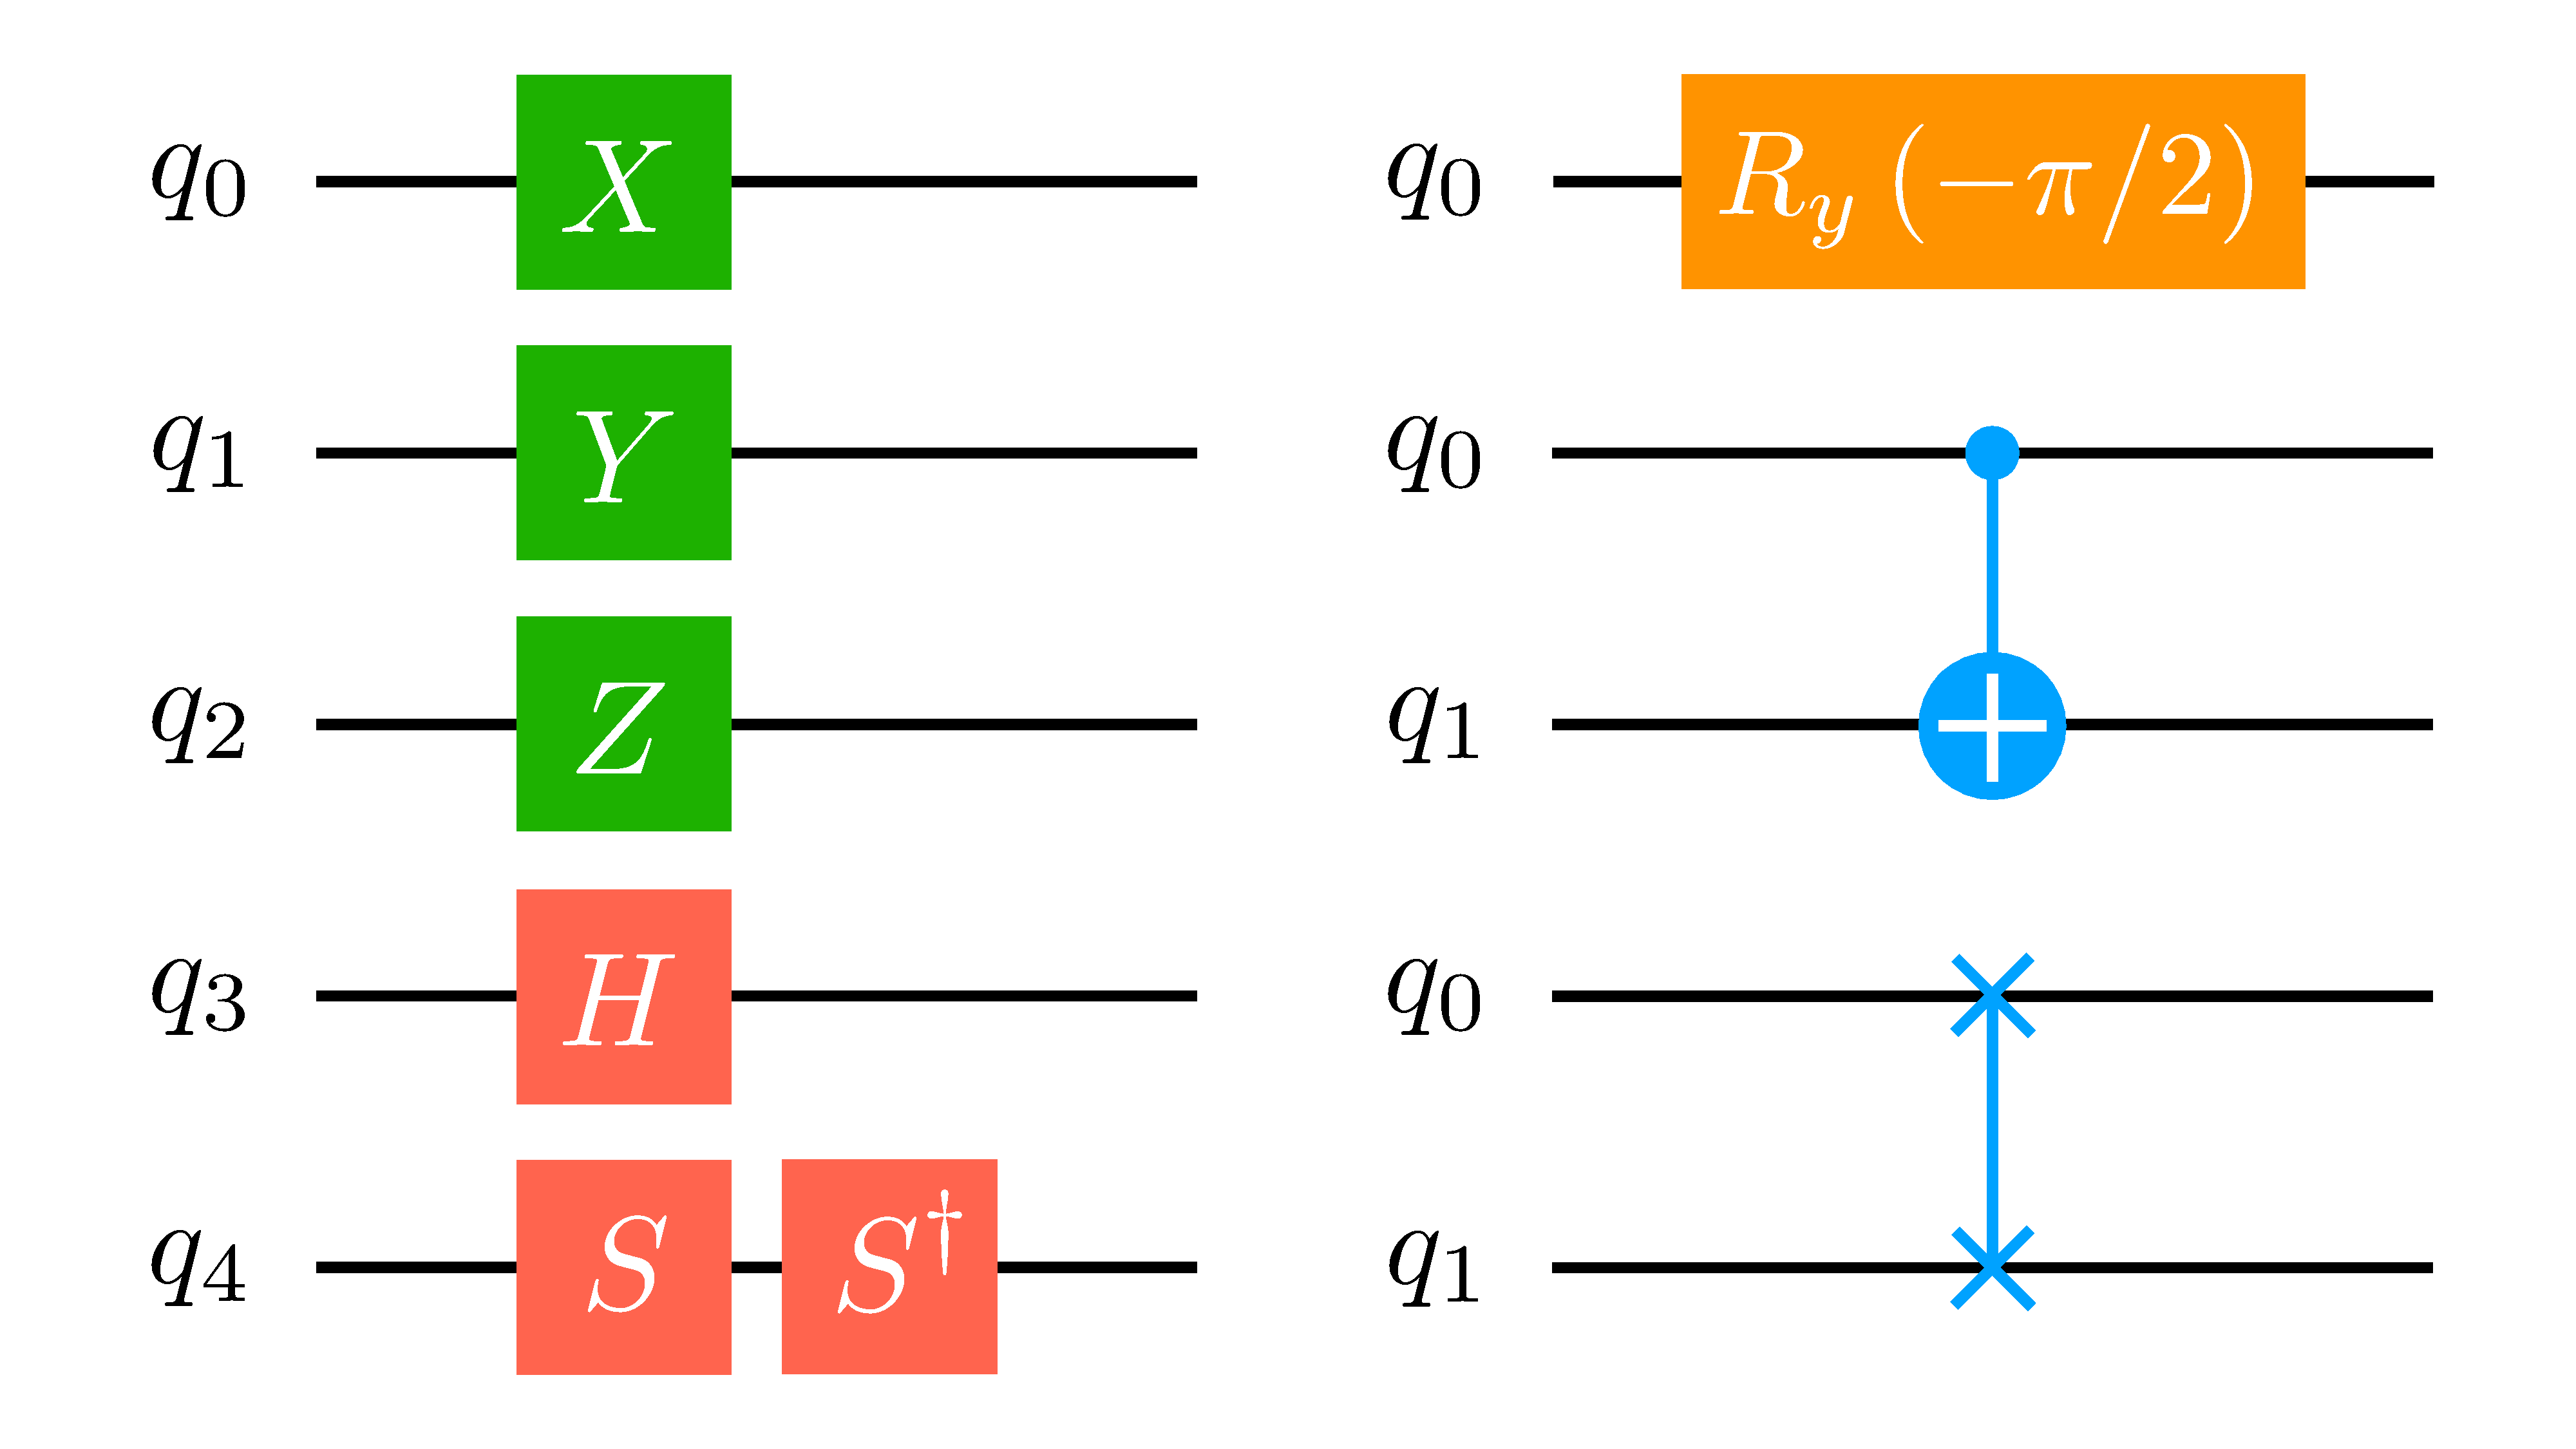
\includegraphics[width=.40\paperwidth]{Figures/quantum-background/circuit-gates-1}
		\end{center}

		\columnbreak

		\begin{center}
			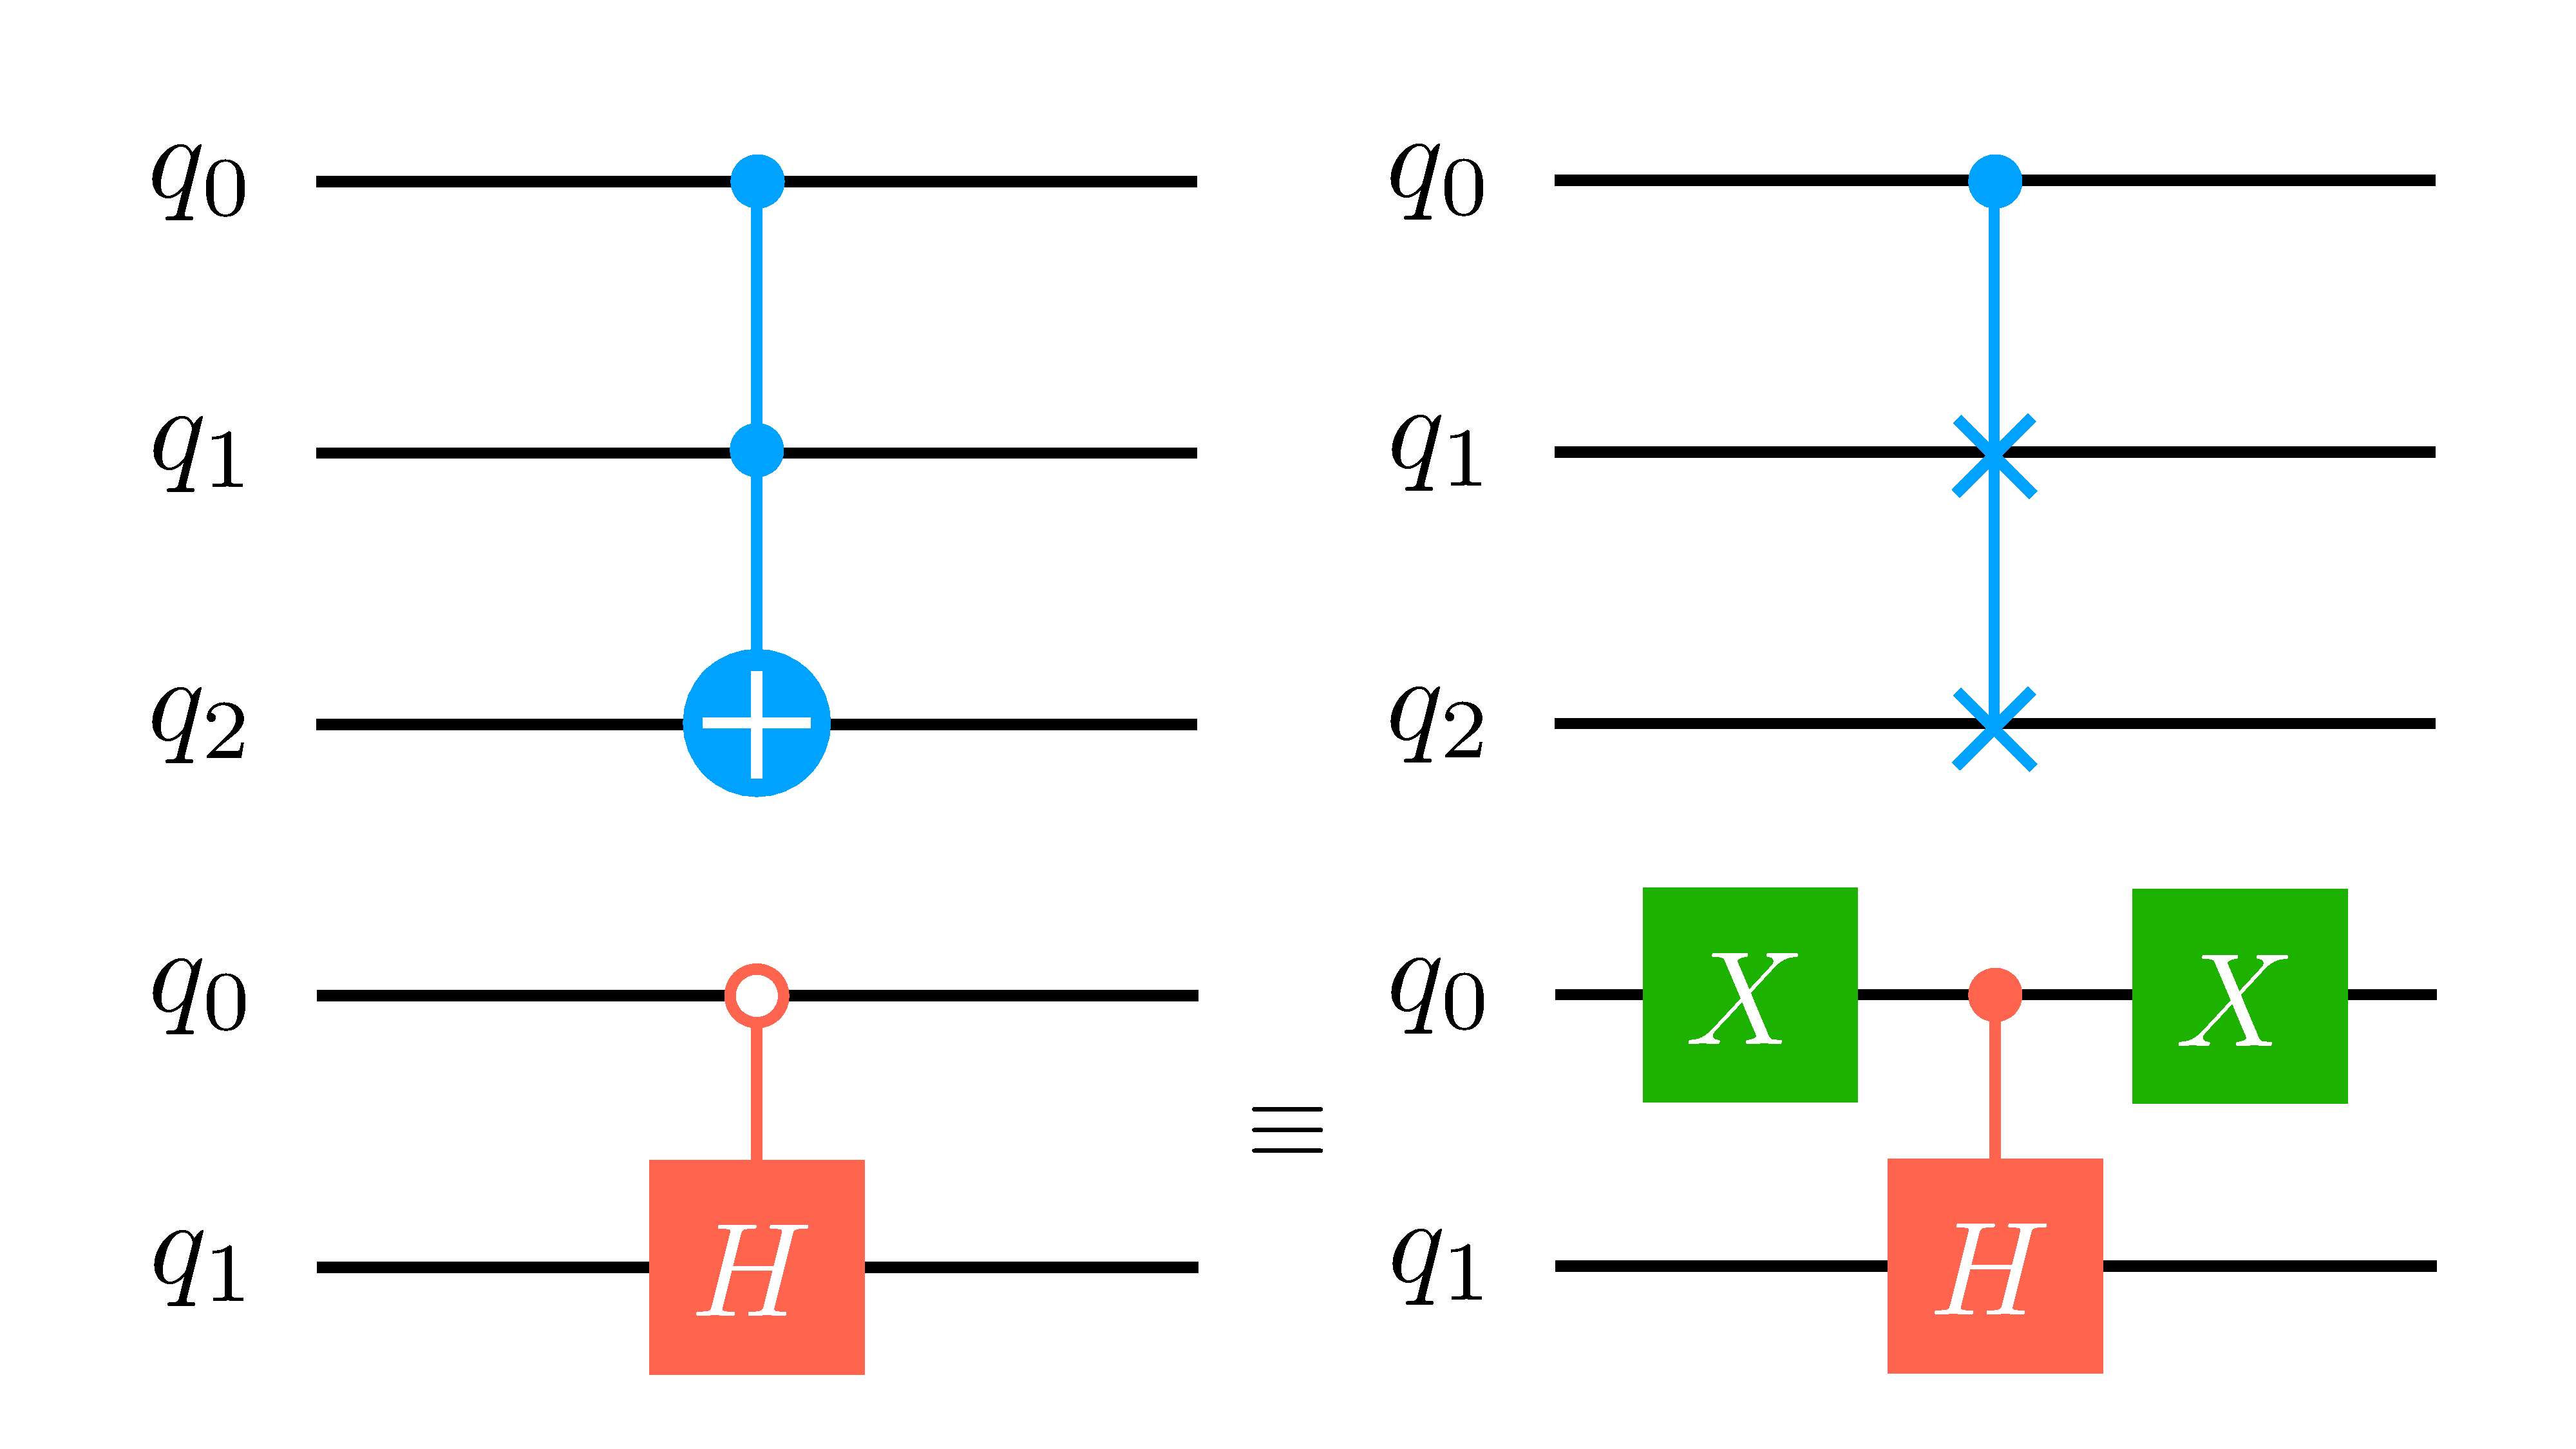
\includegraphics[width=.40\paperwidth]{Figures/quantum-background/circuit-gates-2}
		\end{center}

	\end{multicols}

\end{frame}

%% ----------------------------------------------------------------------------

\begin{frame}{Pauli measurements and the singlet state}

	The final thing that we need to know about are measurements. \textbf{Pauli measurements} are made along the three primary axes of the Bloch sphere, allowing us to calculate the expectation value of \emph{Pauli observables} (i.e. tensor product combinations of the Pauli hermitian operators):

	\begin{multicols}{2}

		\begin{center}
			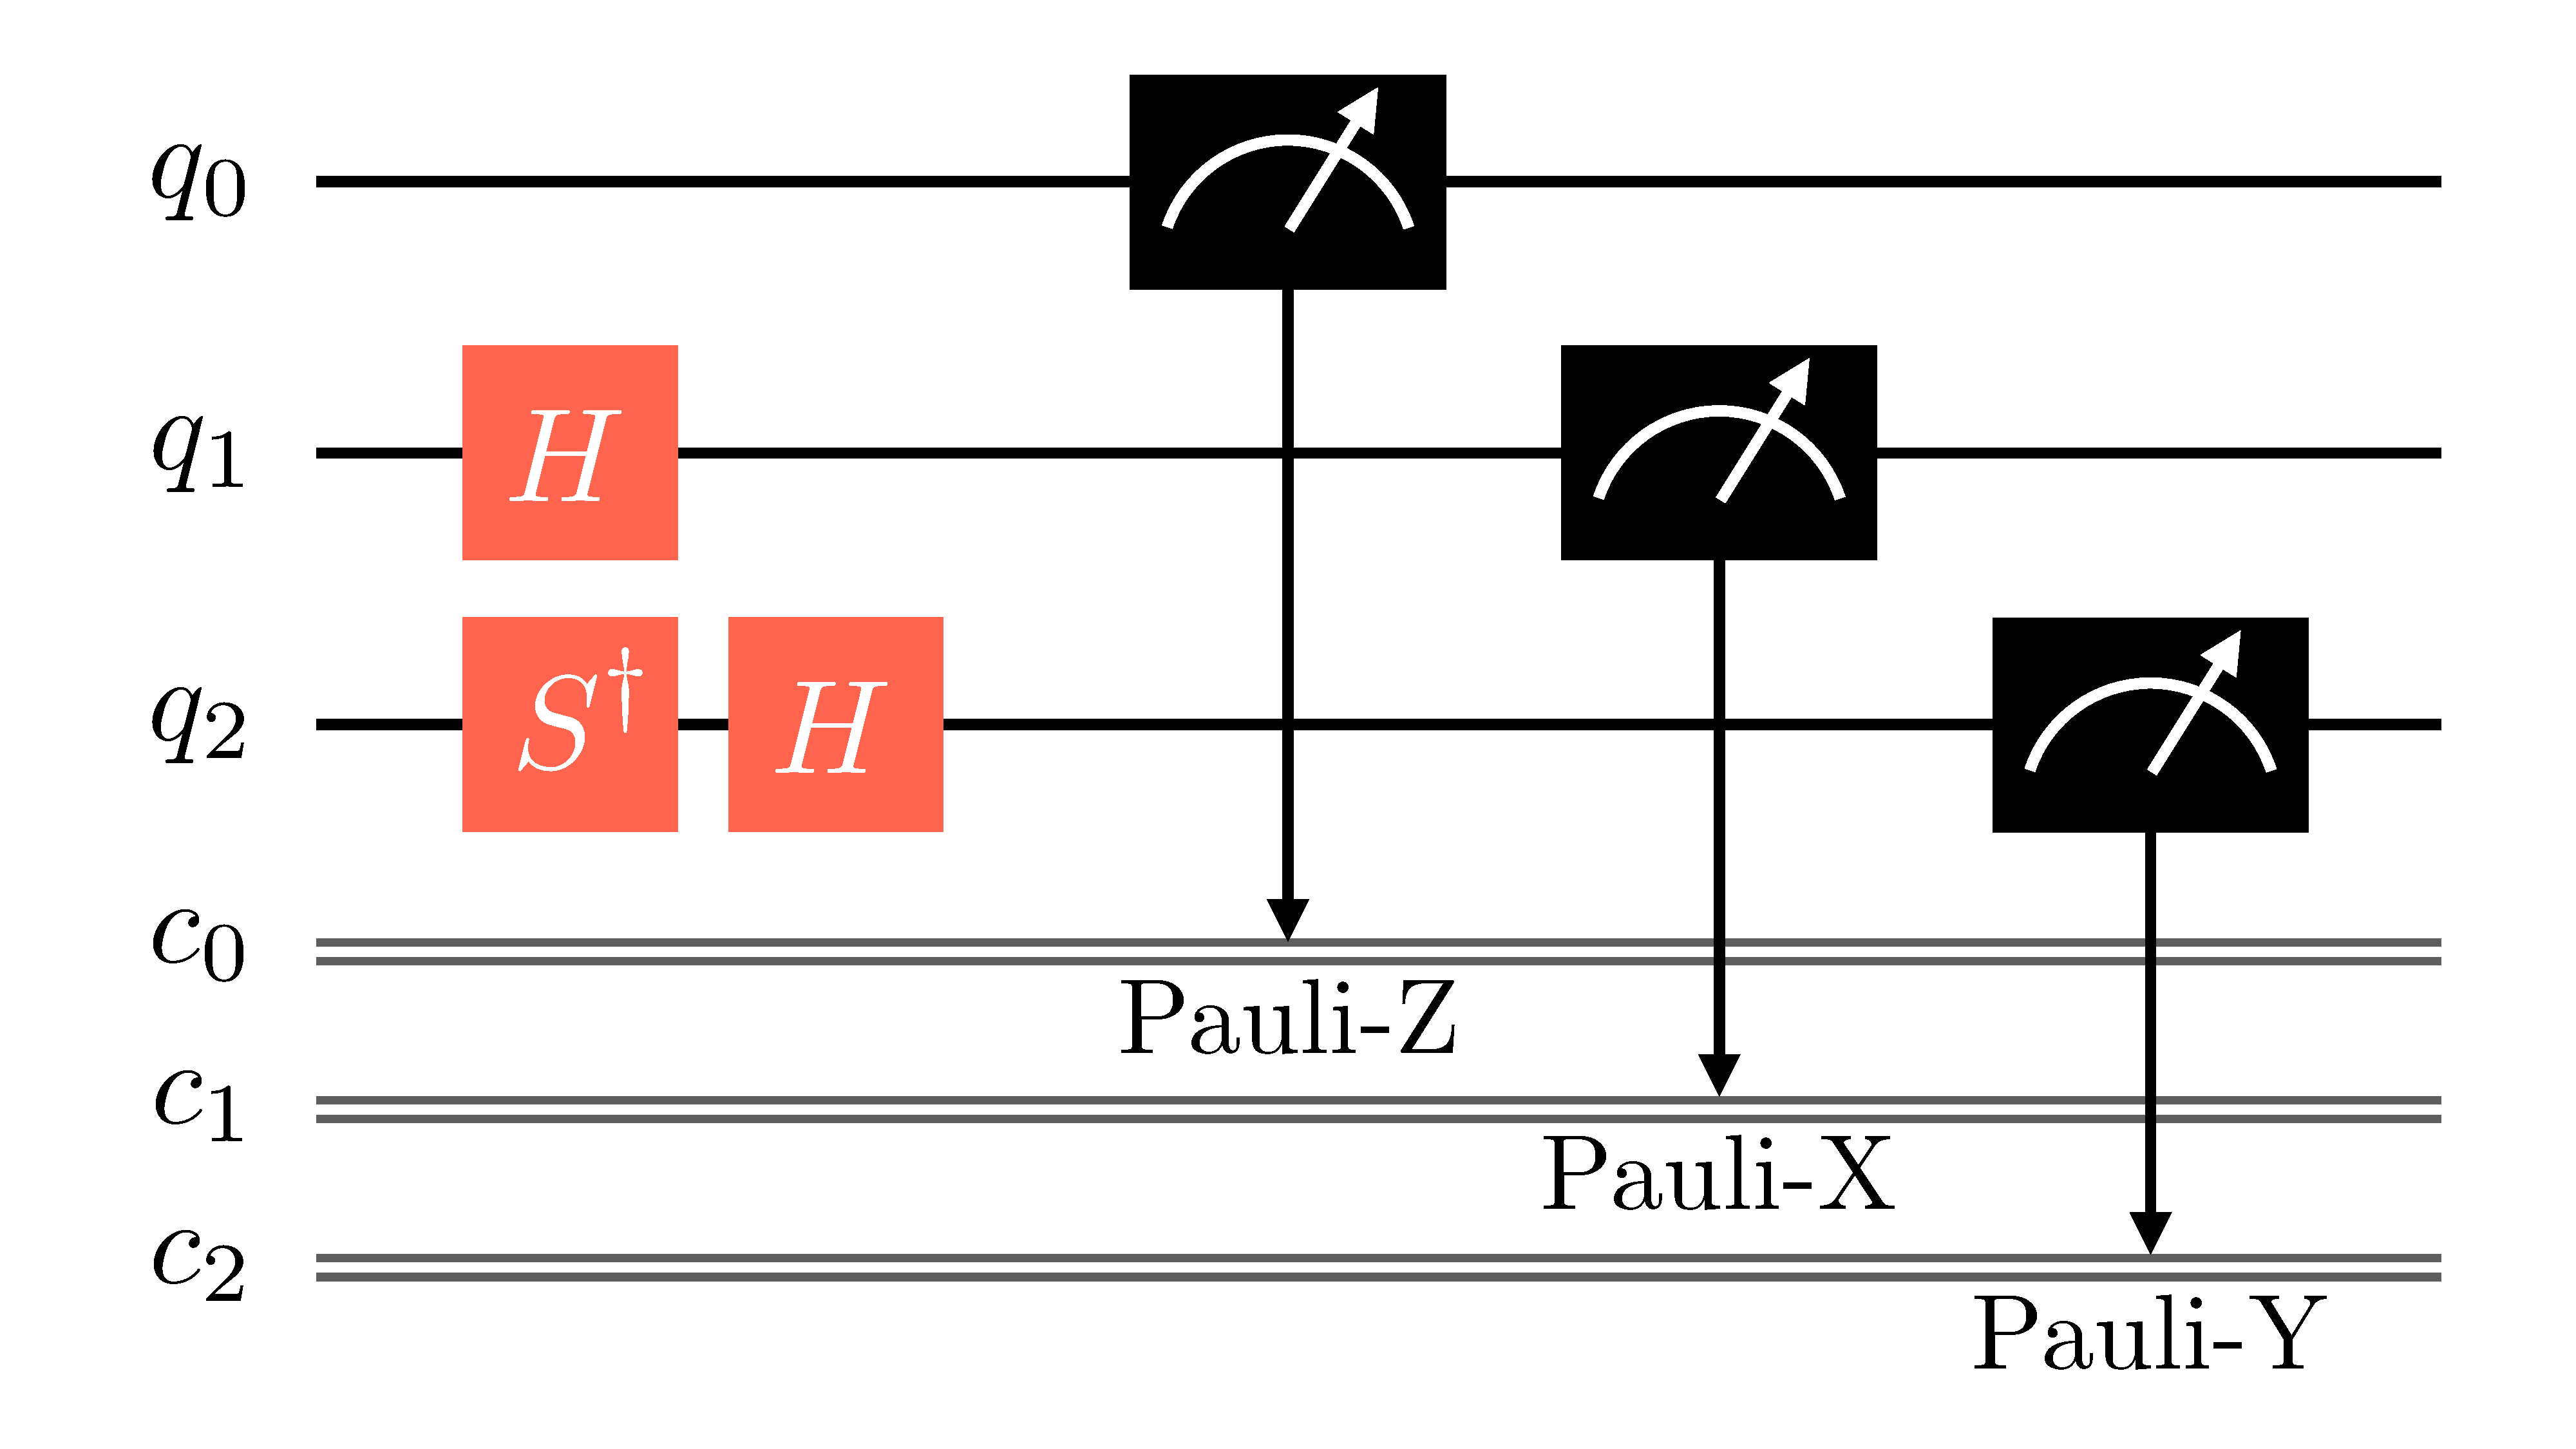
\includegraphics[width=.40\paperwidth]{Figures/quantum-background/circuit-gates-pauli}
		\end{center}

		\columnbreak

		\pause
		\begin{center}
			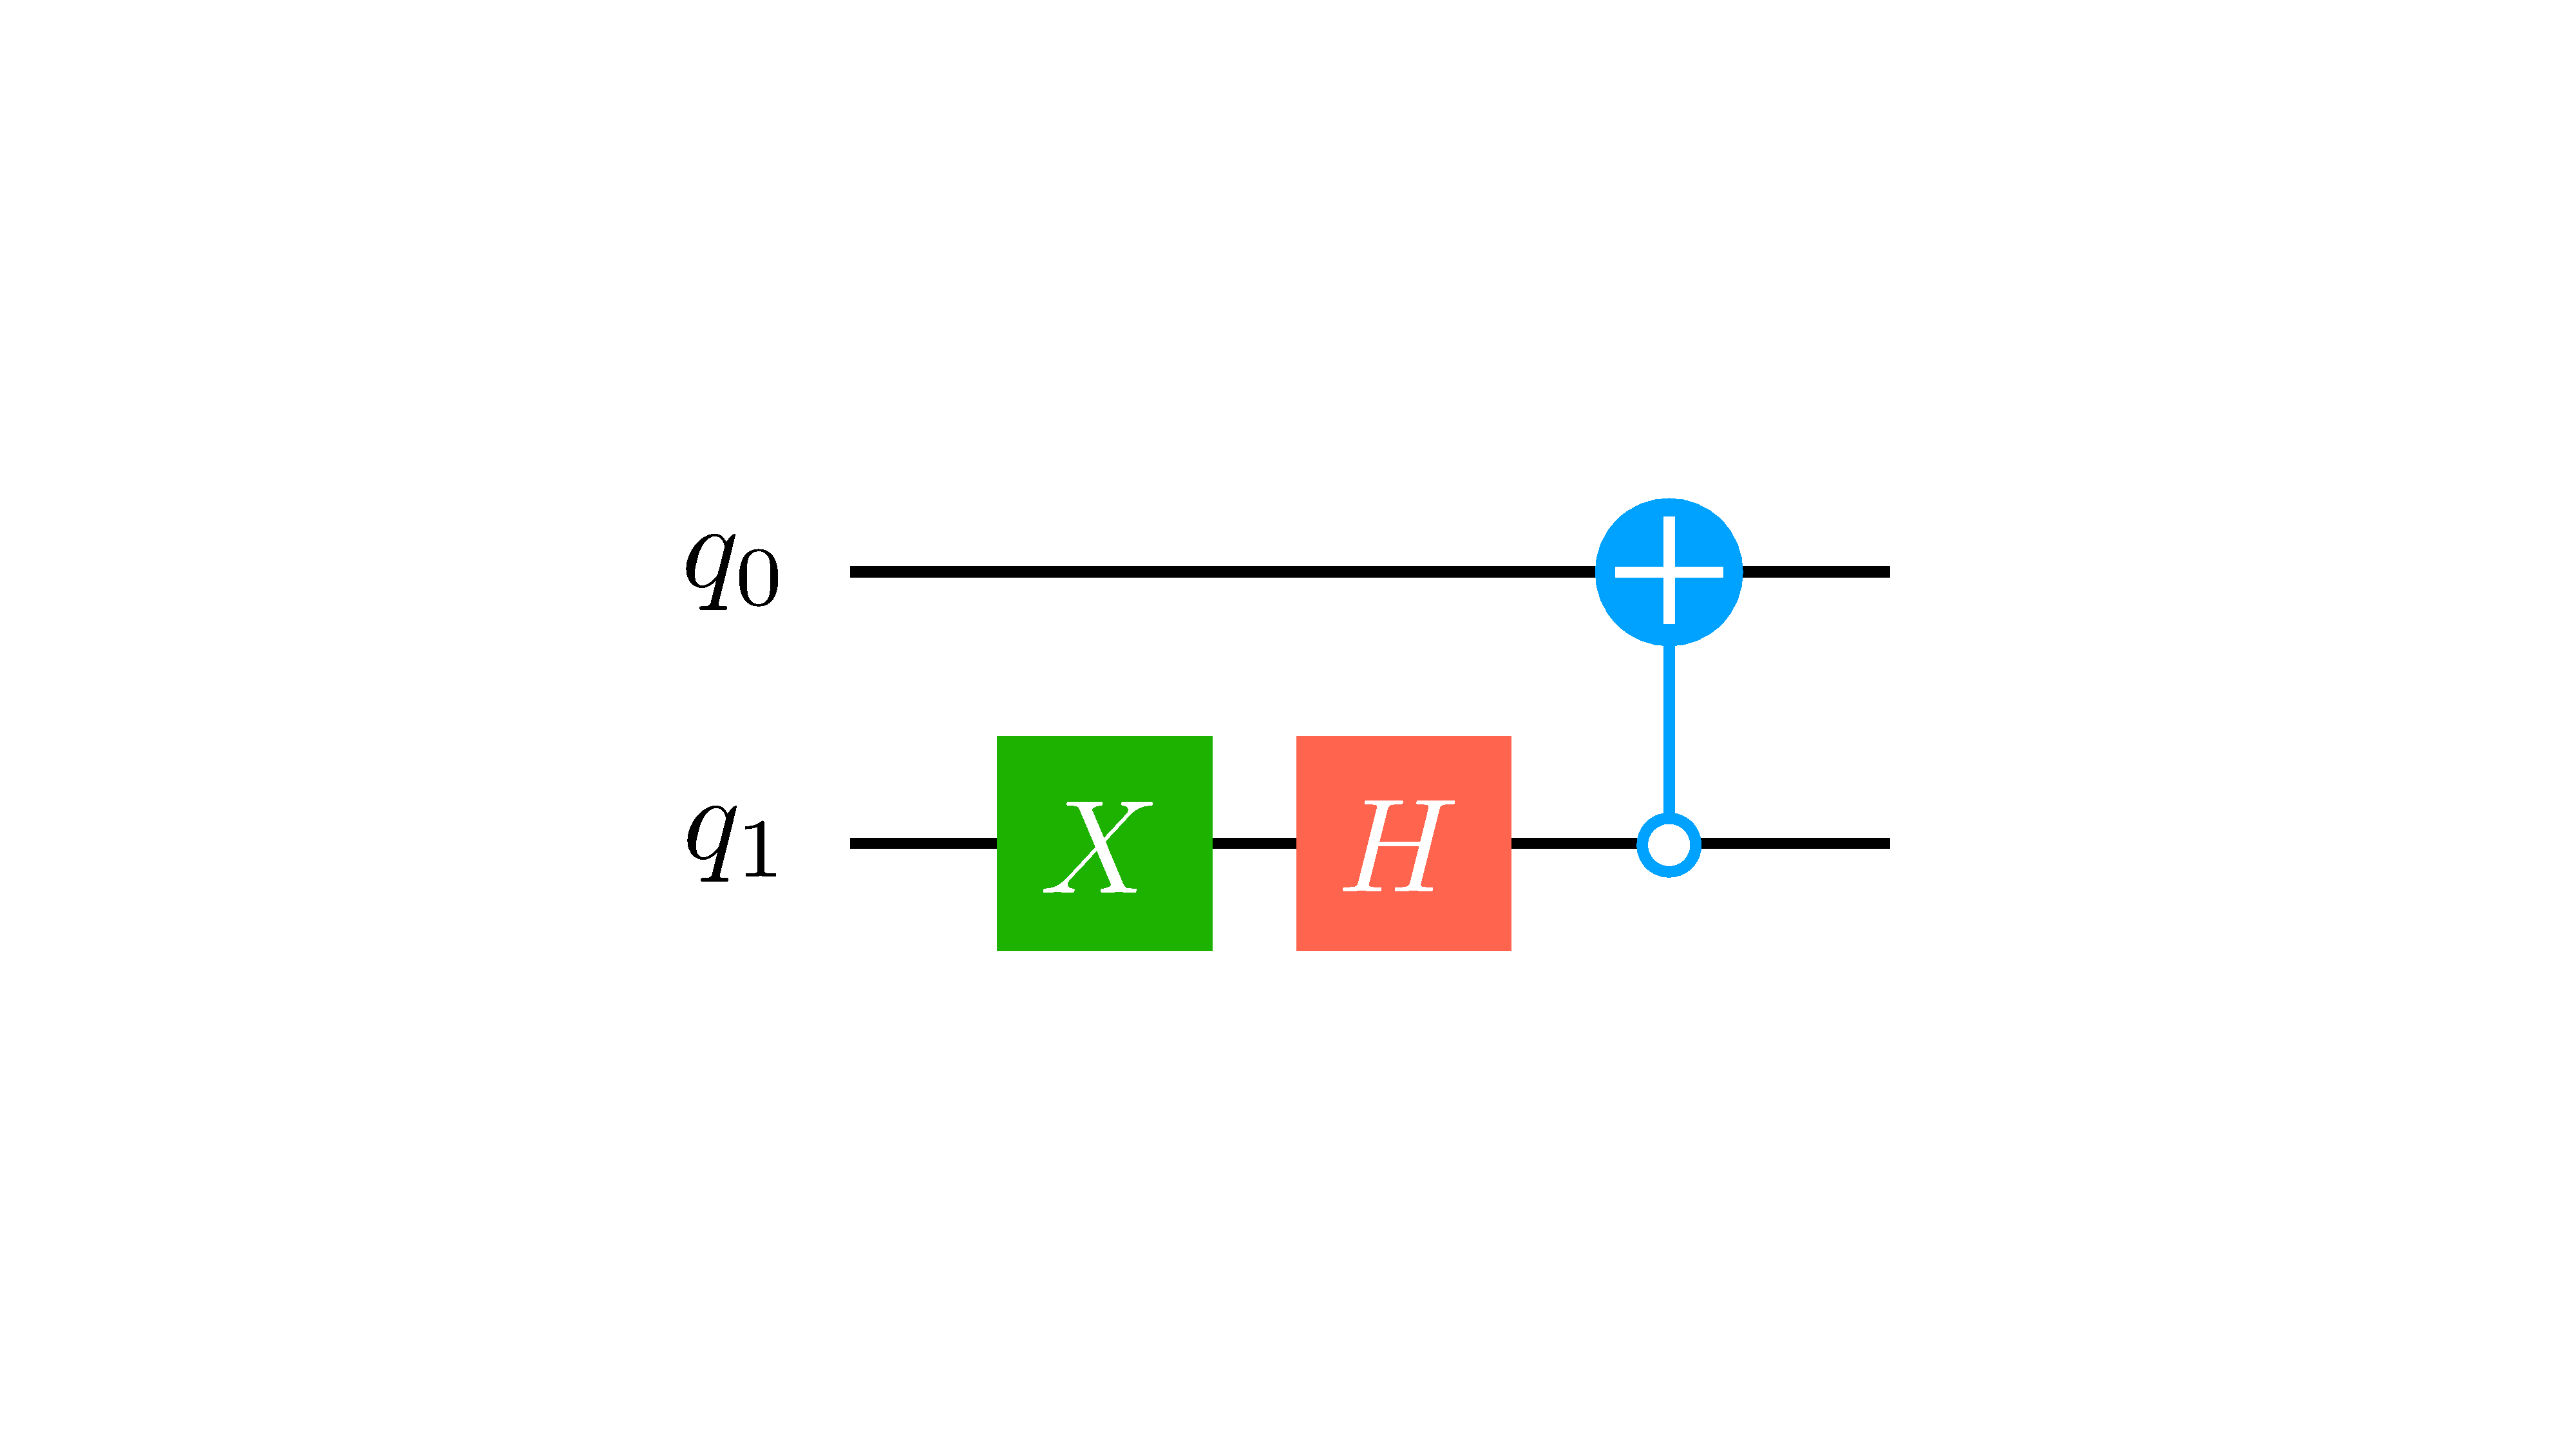
\includegraphics[width=.40\paperwidth]{Figures/quantum-background/circuit-gates-singlet}\\ \vspace{-2em}
			$\ket{\text{\small singlet}} \defeq \frac{\ket{01}-\ket{10}}{\sqrt{2}}$
		\end{center}

	\end{multicols}

\end{frame}

%% ----------------------------------------------------------------------------

\begin{frame}[allowframebreaks]{Deutsch-Jozsa algorithm}

	\begin{multicols}{2}

		\textbf{Deutsch’s problem} says that we are given a function $f: \qty{0,1}^n \ra \qty{0,1}$, and are told that the function is either constant or balanced (i.e. half of the inputs return 0 and the other half 1). The goal is to determine, with the smallest number of evaluations possible, whether the given function is one kind or the other.

		\columnbreak

		\begin{center}
			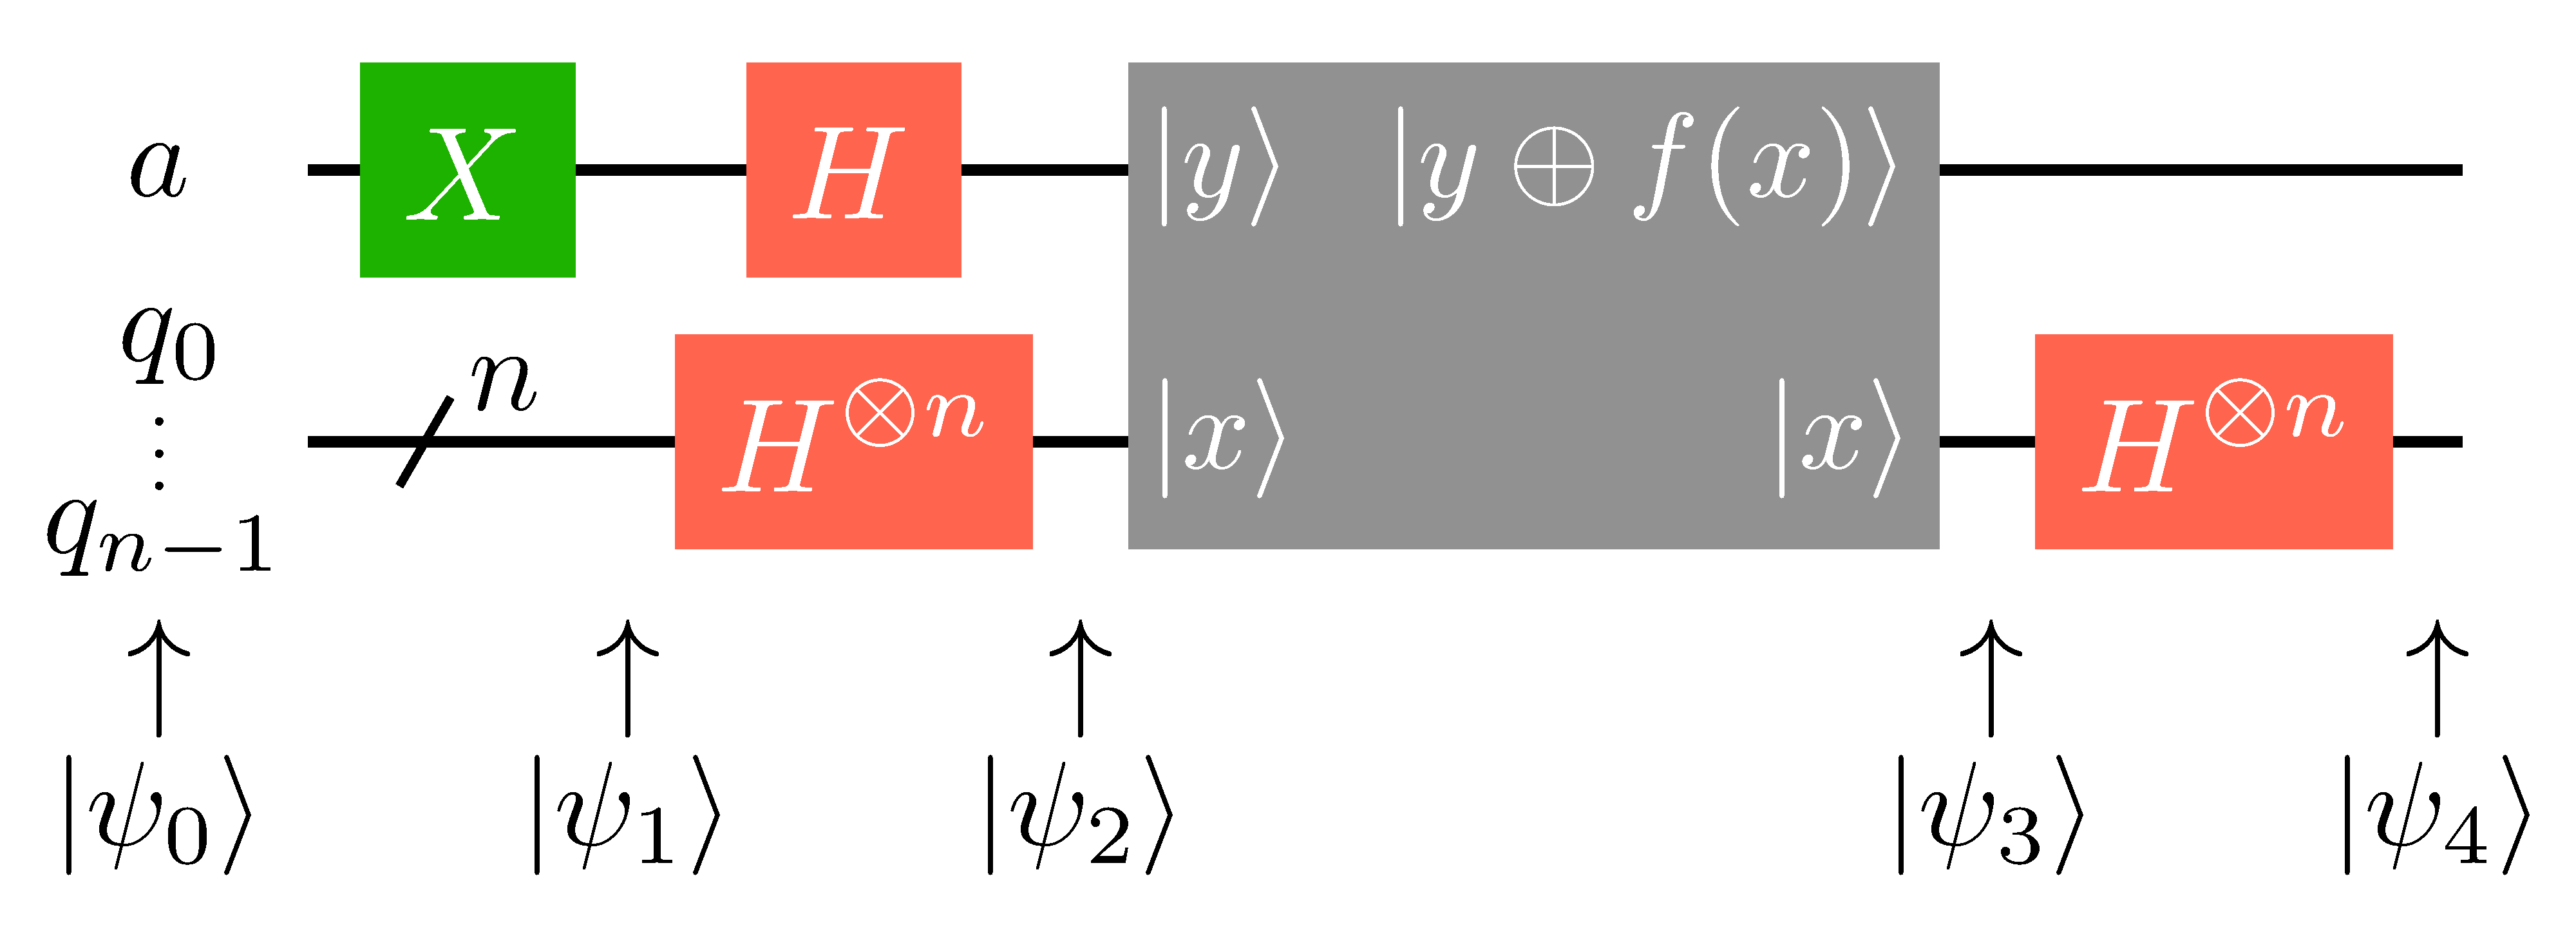
\includegraphics[width=.40\paperwidth]{Figures/quantum-background/deutsch-jozsa-algorithm}
		\end{center}

	\end{multicols}

	Using classical resources the only way to solve this problem is to repeatedly evaluate the function for different inputs. In the worst case scenario, we will need to perform $2^n/2+1$ evaluations, since it is always possible to obtain $2^n/2$ times the same number even if the function is balanced. However, making use of quantum superposition, we can find a way to solve this problem with just one evaluation. The key as to why this is possible is quantum superposition. By evaluating the target function for a superposition state, we are evaluating it simultaneously for all possible inputs. This is sometimes referred to as \textbf{quantum parallelism}.

\break

	The solution to this problem as expressed by the quantum circuit in the previous slide is known as the \textbf{Deutsch-Jozsa algorithm}:

	\begin{multicols}{2}

		\begin{gather*}
		  \ket{\psi_0} = \ket{0}^{\otimes \qty(n+1)} \\[10pt]
		  \ket{\psi_1} = \ket{0}^{\otimes n} \ket{1} \\[10pt]
			H^{\otimes n} \ket{x} =
		    \sum_{z \in \qty{0,1}^n} (-1)^{x \cdot z}
				\frac{\ket{z}}{\sqrt{2^n}} \\[10pt]
			\ket{\psi_2} =
		    \sum_{x \in \qty{0,1}^n} \frac{\ket{x}}{\sqrt{2^n}}
		    \qty[\frac{\ket{0}-\ket{1}}{\sqrt{2}}]
		\end{gather*}

		\columnbreak

		\begin{gather*}
		  \frac{\ket{0 \oplus f(x)}-\ket{1 \oplus f(x)}}{\sqrt{2}} =
		    (-1)^{f(x)} \frac{\ket{0}-\ket{1}}{\sqrt{2}} \\[10pt]
			\ket{\psi_3} =
		    \sum_{x \in \qty{0,1}^n} \frac{(-1)^{f(x)} \ket{x}}{\sqrt{2^n}}
		    \qty[\frac{\ket{0}-\ket{1}}{\sqrt{2}}] \\[10pt]
			\ket{\psi_4} =
		    \sum_{\substack{x \in \qty{0,1}^n \\ z \in \qty{0,1}^n}}
		    \frac{(-1)^{x \cdot z +f(x)} \ket{z}}{2^n}
		    \qty[\frac{\ket{0}-\ket{1}}{\sqrt{2}}]
		\end{gather*}

	\end{multicols}

\end{frame}

%% ----------------------------------------------------------------------------

\begin{frame}[allowframebreaks]{Quantum Fourier transform}

	The usual \textbf{Discrete Fourier Transform} (DFT) can be expressed as:

	\medskip

	\begin{align*}
	  \ket{j} \qra&
				\frac{1}{\sqrt{N}} \sum_{k=0}^{N-1} \exp[2\pi i \frac{jk}{N}] \ket{k} \\
	    =& \frac{1}{2^{n/2}} \sum_{k_{n-1}=0}^{1} \cdots \sum_{k_{0}=0}^{1}
	      \exp[2\pi ij \qty(\sum_{l=0}^{n-1} k_{l} 2^{l-n})]
	      \ket{\bin k_{n-1} \dots k_{0}} \\
	    =& \frac{1}{2^{n/2}} \sum_{k_{n-1}=0}^{1} \cdots \sum_{k_{0}=0}^{1}
	      \qty{ \bigotimes_{l=1}^{n} \exp[2\pi ij k_{n-l} 2^{-l}]
	      \ket{k_{n-l}} } \\
	    =& \frac{1}{2^{n/2}} \bigotimes_{l=1}^{n}
	      \qty{ \sum_{k_{n-l}=0}^{1} \exp[2\pi ij k_{n-l} 2^{-l}] \ket{k_{n-l}} }
	    = \frac{1}{2^{n/2}} \bigotimes_{l=1}^{n}
	      \qty{ \ket{0} + \exp[2\pi ij 2^{-l}] \ket{1} }
	\end{align*}

\break

	\begin{gather*}
		\ket{j} \ra
			\frac{
				\qty{\ket{0}+ e^{2\pi i \qty(\bin.j_{0})} \ket{1}} \otimes
				\qty{\ket{0}+ e^{2\pi i \qty(\bin.j_{1}j_{0})} \ket{1}} \otimes
				\cdots \otimes
				\qty{\ket{0} + e^{2\pi i \qty(\bin.j_{n-1}j_{n-2} \dots j_{0})} \ket{1}}
			}{2^{n/2}} \\[10pt]
		R_{k} \defeq \mqty[1 & 0 \\ 0 & e^{2\pi i/2^k}]
	\end{gather*}

	\vspace{-2em}

	\begin{center}
		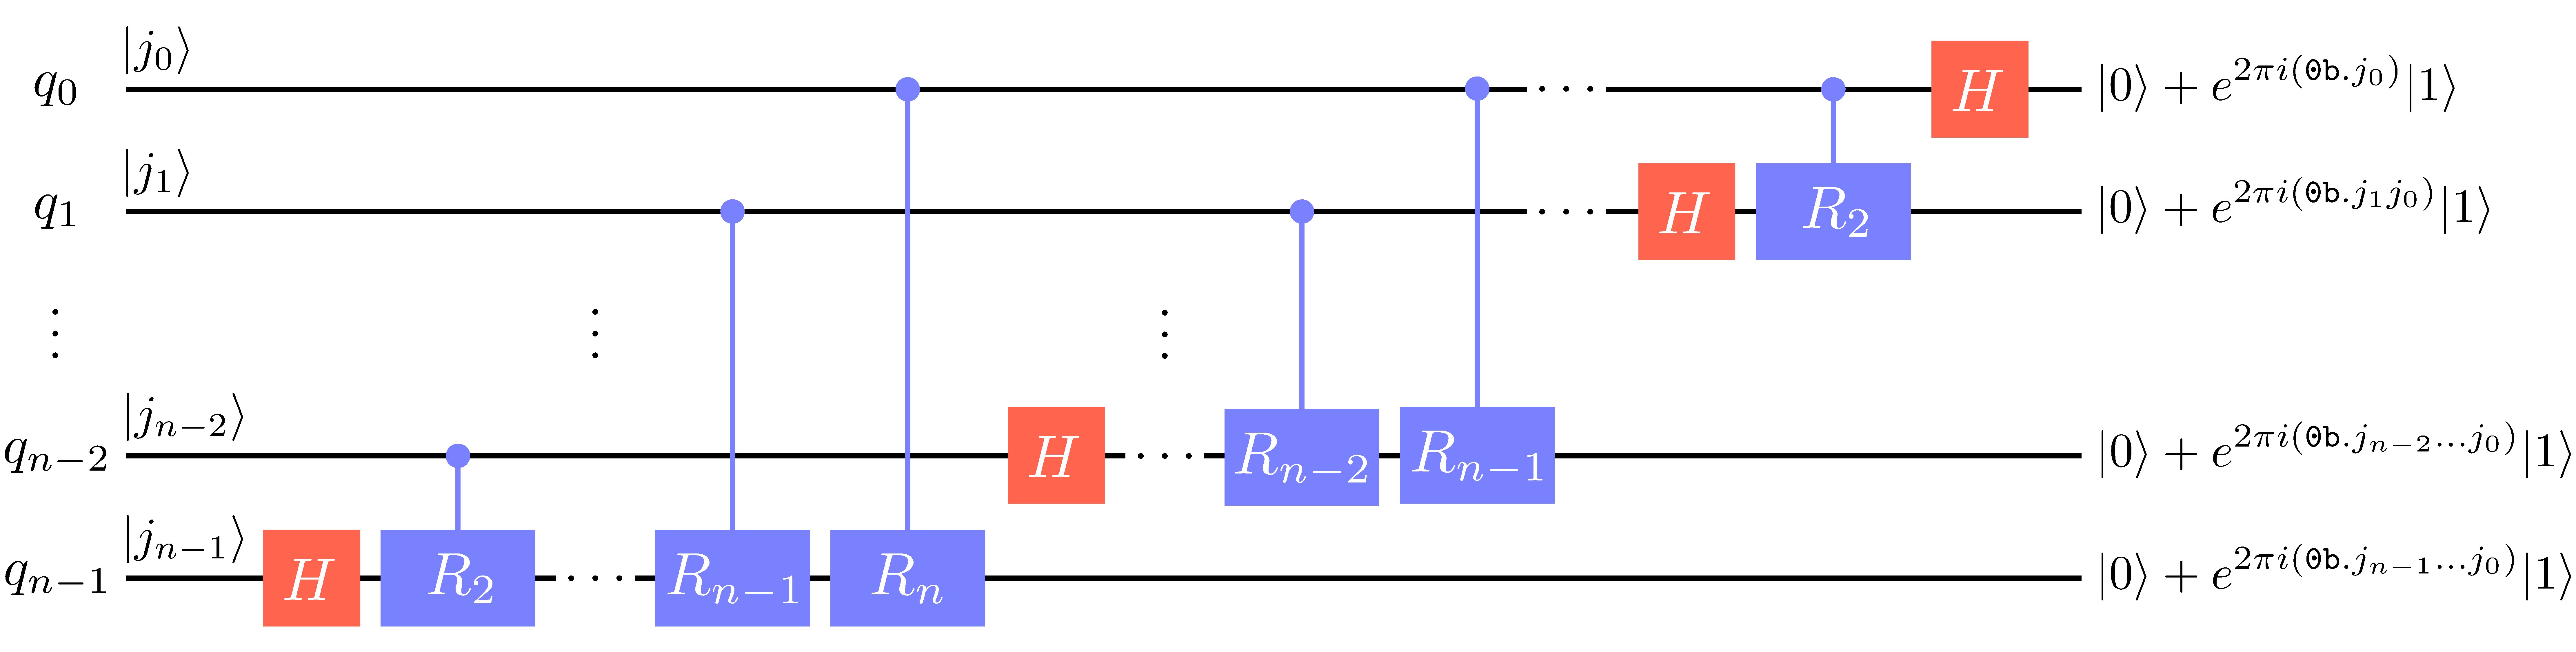
\includegraphics[width=.80\paperwidth]{Figures/quantum-background/quantum-fourier-transform}
	\end{center}

\break

	We can now compare the complexity of this algorithm with its best classical counterparts. This is done by counting the number of gates in the circuit, where we have to remember the final SWAP gates omitted in the representation.

	\begin{multicols}{2}
	\begin{centering}

		\underline{\textbf{FAST FOURIER TRANSFORM}}\\
		\medskip
		$N\log_2 N \equiv \Theta\qty(n2^n)$

		\columnbreak

		\underline{\textbf{QUANTUM FOURIER TRANSFORM}}\\
		\medskip
		$\sum_{k=1}^{n}k + \frac{n}{2} =
			\frac{n\qty(n+1)}{2} + \frac{n}{2} \equiv \Theta\qty(n^2)$

	\end{centering}
	\end{multicols}

	Nonetheless, this technique cannot be used directly for computing the target transform; since we do not know how to recover the individual amplitudes from the quantum states. On top of that, there is no efficient general method for preapring the states to be transformed. This is a great example of an algorithm that presents huge savings compared to its classical analogs, but which cannot be generally used as much as we would like to due to our inability to extract the desirerd information. In some instances however, we can profit from this method to great deeds ---mainly as part of bigger algorithms. An important application is \textbf{Shor's factoring algorithm}, which can be used for efficiently finding the prime decomposition of any given number.

\end{frame}

%% ----------------------------------------------------------------------------

\subsection{Applications}

\begin{frame}{Applications}

	Generally speaking, quantum computing is thought to be able to outperform classical processors, but not for all tasks. This raises the important question of determining which problems are easy to solve using quantum logic while remaining hard for classical approaches. As a matter of fact, we do not fully understand the extent to which there are problems of this kind; and many of the ones we suspect to be good candidates have no formal proof to back them up.\pause~So far, some of the applications that have been found are:

	\begin{multicols}{3}

		\begin{itemize}
			\item Cryptography
			\item Secure communications
			\item Quantum randomness
		\end{itemize}

		\columnbreak

		\begin{itemize}
			\item Quantum sensing
			\item Optimization
			\item Algebra
		\end{itemize}

		\columnbreak

		\begin{itemize}
			\item Machine learning
			\item Quantum games
			\item Quantum simulation
		\end{itemize}

	\end{multicols}

	\pause

	Quantum physics ---especially Quantum Field Theory--- is the ideal place to look for (relevant) problems which can be solved on a quantum computer while remaining intractable for classical machines; that also makes it the best choice for analyzing the computational power behind this new paradigm.

\end{frame}


%% ----------------------------------------------------------------------------
%% ----------------------------------------------------------------------------

\section{Solving the NJL model in $1+1$ dimensions}

\begin{frame}{Solving the NJL model in $1+1$ dimensions}

	The NJL \textbf{Lagrangian density} that we will make use of looks like:

	\begin{gather*}
		\mathcal{L}(x) =
	    \bar{\psi}(x) \qty(i\slashed{\partial}-m) \psi(x) + \mathcal{L}_{I}(x) \\[10pt]
		\mathcal{L}_{I}(x) =
	    \frac{1}{2} G_{\pi} \qty[\bar{\psi}(x)\psi(x)]^2
	\end{gather*}

	From this expression for the Lagrangian density we can obtain the corresponding \textbf{Hamiltonian density} through the Legendre transform. In special, for $1+1$ dimensions:

	\begin{align*}
	  \mathcal{H} &\defeq
	    \fdv{\mathcal{L}}{\qty(\partial_{0} \psi)} \qty(\partial_{0} \psi) +
	    \qty(\partial_{0} \bar{\psi})
	    \fdv{\mathcal{L}}{\qty(\partial_{0} \bar{\psi})} -
	    \mathcal{L} \\
	  &= \bar{\psi}(x)\qty(m - i\gamma^{1}\partial_{1})\psi(x) -
    	\frac{1}{2} G_{\pi} \qty[\bar{\psi}(x)\psi(x)]^{2}
	\end{align*}

\end{frame}

%% ----------------------------------------------------------------------------

\subsection{Analytical solution}

\begin{frame}{Dressed mass and the gap equation}

	\begin{multicols}{2}

		The \textbf{bare and dressed masses} appear on the bare quark propagator $S_{0}$, and the NJL dressed quark propagator $S$ respectively:

		\vspace{1em}

		\begin{gather*}
		  S_0^{-1} \defeq \slashed{p} - m + i\varepsilon \\[5pt]
		  S^{-1} \equiv S^{-1}_\text{\tiny NJL} \defeq \slashed{p} - M + i\varepsilon
		\end{gather*}

		\columnbreak

		\begin{center}
			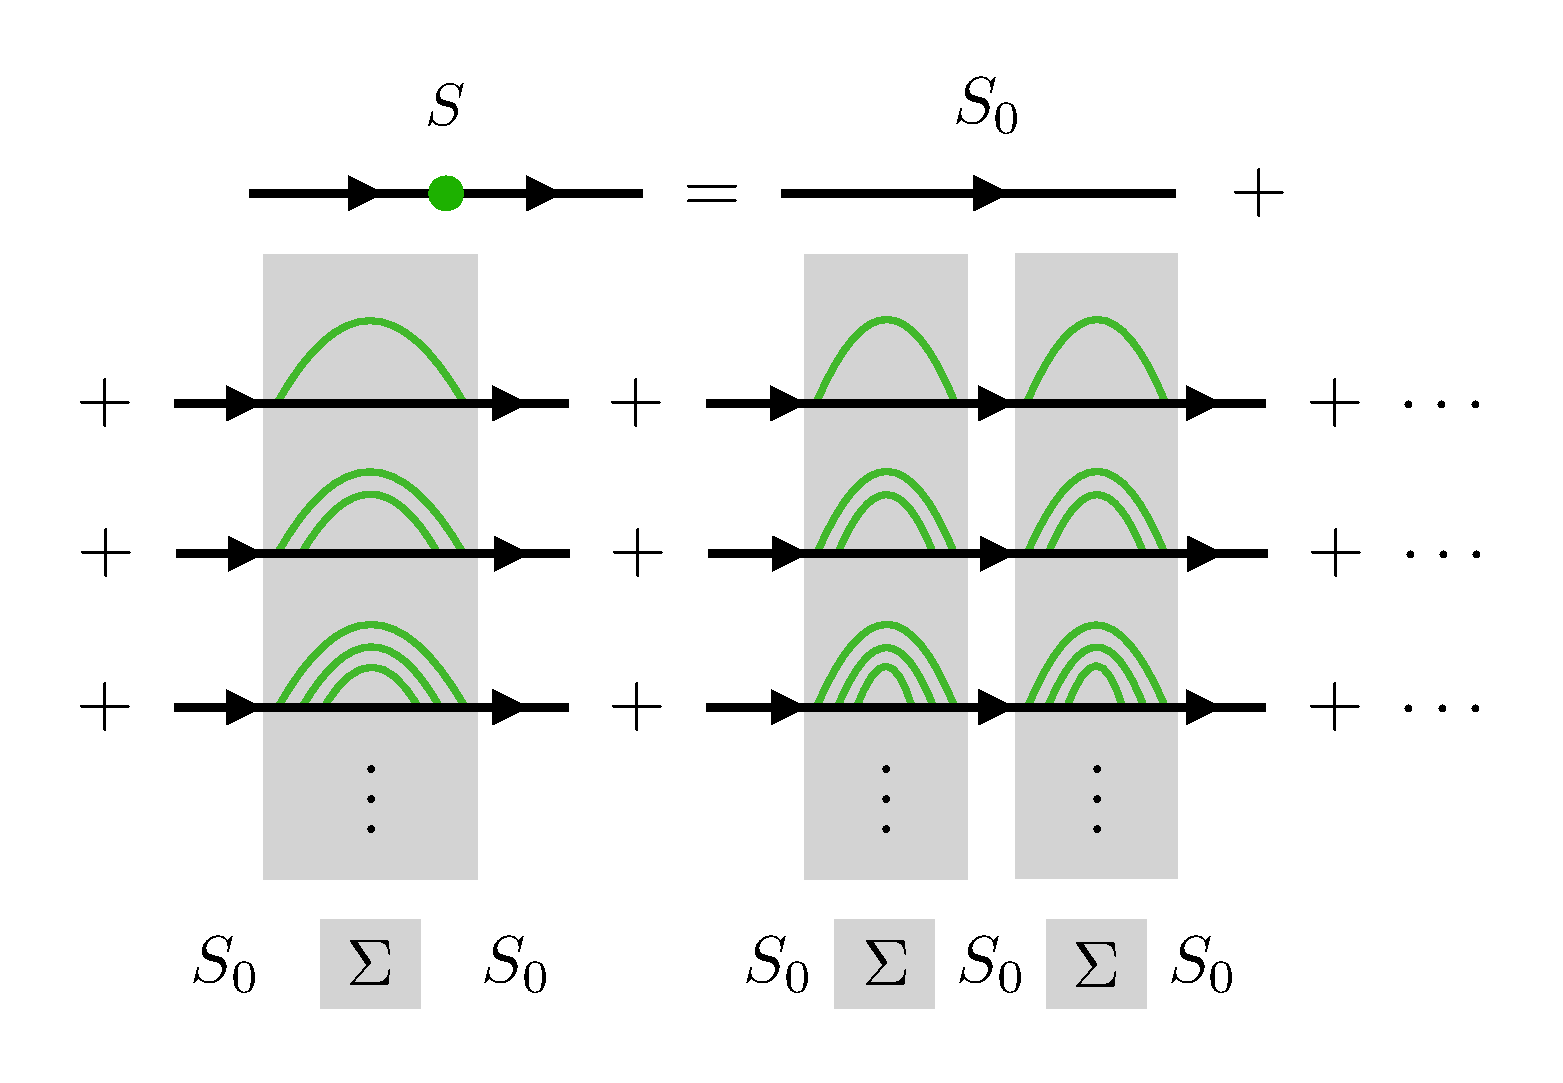
\includegraphics[width=.30\paperwidth]{Figures/NJL1-model-solving/gap-equation}
		\end{center}

	\end{multicols}

	We can find a relationship between these two by solving the \textbf{gap equation}:

	\begin{gather*}
		S^{-1} =
			S_{0}^{-1} - 2iG_{\pi} \int \frac{\dd[2]{p}}{\qty(2\pi)^{2}}
			N_\text{color} N_\text{flavor} \text{Tr}_\text{\tiny{D}}\qty[S] \\
	  M \simeq
	    m + 4iG_\pi N_\text{color} N_\text{flavor}
	    \int \frac{\dd[2]{p}}{(2\pi)^2} \frac{M}{p^2 - M^2}
	\end{gather*}

\end{frame}

%% ----------------------------------------------------------------------------

\begin{frame}[allowframebreaks]{Mass generation}

	To solve this last expression we first perform a \textbf{Wick rotation} $p_0 \ra i p_2 \qRa (p_0)^2 \ra - (p_2)^2$, followed by a transformation to \textbf{polar coordinates}:

	\begin{gather*}
		M \simeq
	    m + N_\text{color}  N_\text{flavor}
	    \frac{G_\pi}{\pi} \int_{0}^{\infty} \frac{M}{p_E^2 + M^2} \dd{p_E^2}
	\end{gather*}

	Finally, to make the integral converge, we introduce \textbf{proper time regularization}:

	\begin{gather*}
	  \frac{1}{x^n} =
	    \frac{1}{(n-1)!} \int_{0}^{\infty} \dd{\tau} \tau^{n-1} \exp[-\tau x] \ra
	    \frac{1}{(n-1)!} \int_{1/\Lambda_{UV}^2}^{1/\Lambda_{IR}^2}
	      \dd{\tau} \tau^{n-1} \exp[-\tau x] \\[5pt]
	  M \simeq
	    m + M N_\text{color} N_\text{flavor} \frac{G_\pi}{\pi}
	    \int_{1/\Lambda_{UV}^2}^{1/\Lambda_{IR}^2} \frac{\dd{\tau}}{\tau}
	    \exp[-\tau M^{2}]
	\end{gather*}

	Where $\Lambda_{IR}$ and $\Lambda_{UV}$ are the \textbf{infrared and ultraviolet cutoffs} respectively.

\break

	\begin{center}
		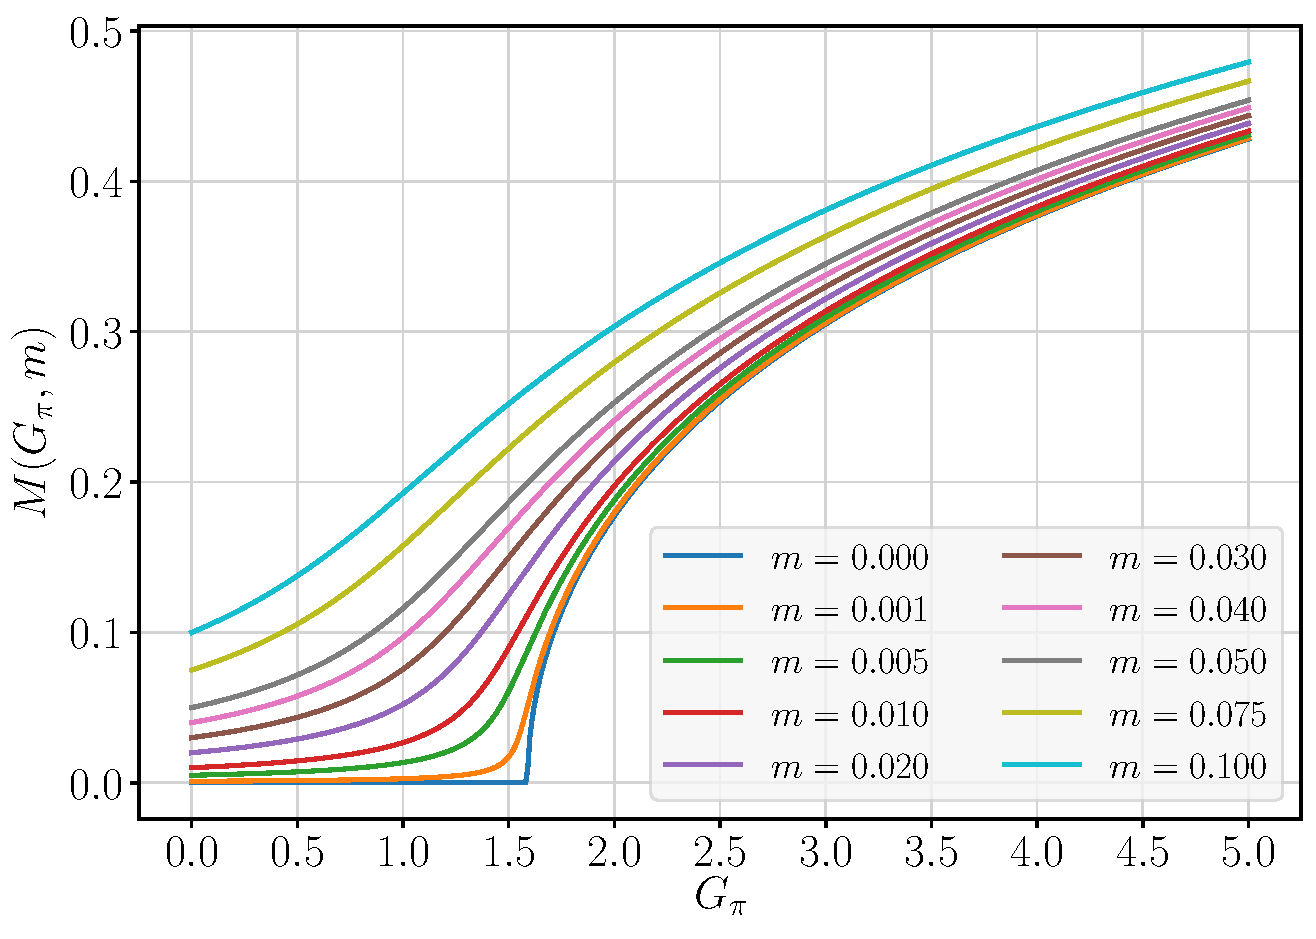
\includegraphics[width=.5\paperwidth]{Figures/NJL1-model-solving/NJL1-dressed-mass-curves}
	\end{center}

	\vspace{-1em}

	\begin{table}[!bp]
	  \centering
	  % \caption{Parameters used for solving the NJL model in $1+1$ dimensions.}
	  \label{tab:NJL1-analytical-solution-parameters}
	  \begin{tabular}{ c c c c c }
	    \hline
	    % \rule{0pt}{14pt}
	    $N_\text{Dirac}$ & $N_\text{color}$ & $N_\text{flavor}$ &
	    $\Lambda_{IR}$ & $\Lambda_{UV}$ \\
	    \hline
	    \hline
	    % \rule{0pt}{14pt}
	    $1+1 \ra 2$ & $1$ & $1$ & $0.240$ GeV & $0.645$ GeV \\
	    \hline
	  \end{tabular}
	\end{table}

\end{frame}

%% ----------------------------------------------------------------------------

\subsection{Lattice formulation}

\begin{frame}[allowframebreaks]{Lattice formulation}

	We can define the Hamiltonian of the system as the integral over space of the Hamiltonian density:

	\begin{gather*}
	  H = \int \mathcal{H}(x) \dd{x}
	    = \int \qty{\bar{\psi}(x)\qty(m-i\gamma^{1}\partial_{1})\psi(x) -
	                \frac{1}{2}G_{\pi}\qty[\bar{\psi}(x)\psi(x)]^{2}} \dd{x}
	\end{gather*}

	For a basis where:

	\begin{gather*}
		\psi = \mqty[\psi_{+} \\ \psi_{-}] \qc
	  \bar{\psi} \defeq \psi^{\dagger}\gamma^{0} \qc
		\gamma^{0} = \mqty[1 & 0\\ 0 & -1] \qc
	  \gamma^{1} = \mqty[0 & -1\\ 1 & 0]
	\end{gather*}

	We can write the kinetic term as:

	\begin{gather*}
	  \bar{\psi}\qty(-i\gamma^{1}\partial_{1})\psi =
			\frac{i}{2} \qty{
	      \qty[ \psi^{\dagger}_{+} \qty(\partial_{1}\psi_{-}) -
	      \qty(\partial_{1}\psi^{\dagger}_{+}) \psi_{-} ] +
	      \qty[ \psi^{\dagger}_{-} \qty(\partial_{1}\psi_{+}) -
	      \qty(\partial_{1}\psi^{\dagger}_{-}) \psi_{+} ]
	    }
	\end{gather*}

\break

	The two groups in brackets are essentially equivalent to one another by virtue of exchanging positive and negative energy components. This is the motivation behind \textbf{staggered fermion lattices}, which use two computational lattice sites for each theoretical value of $\psi$.

	\begin{figure}[!tbp]
		\centering
		\begin{minipage}[c]{.45\linewidth}
			\centering
			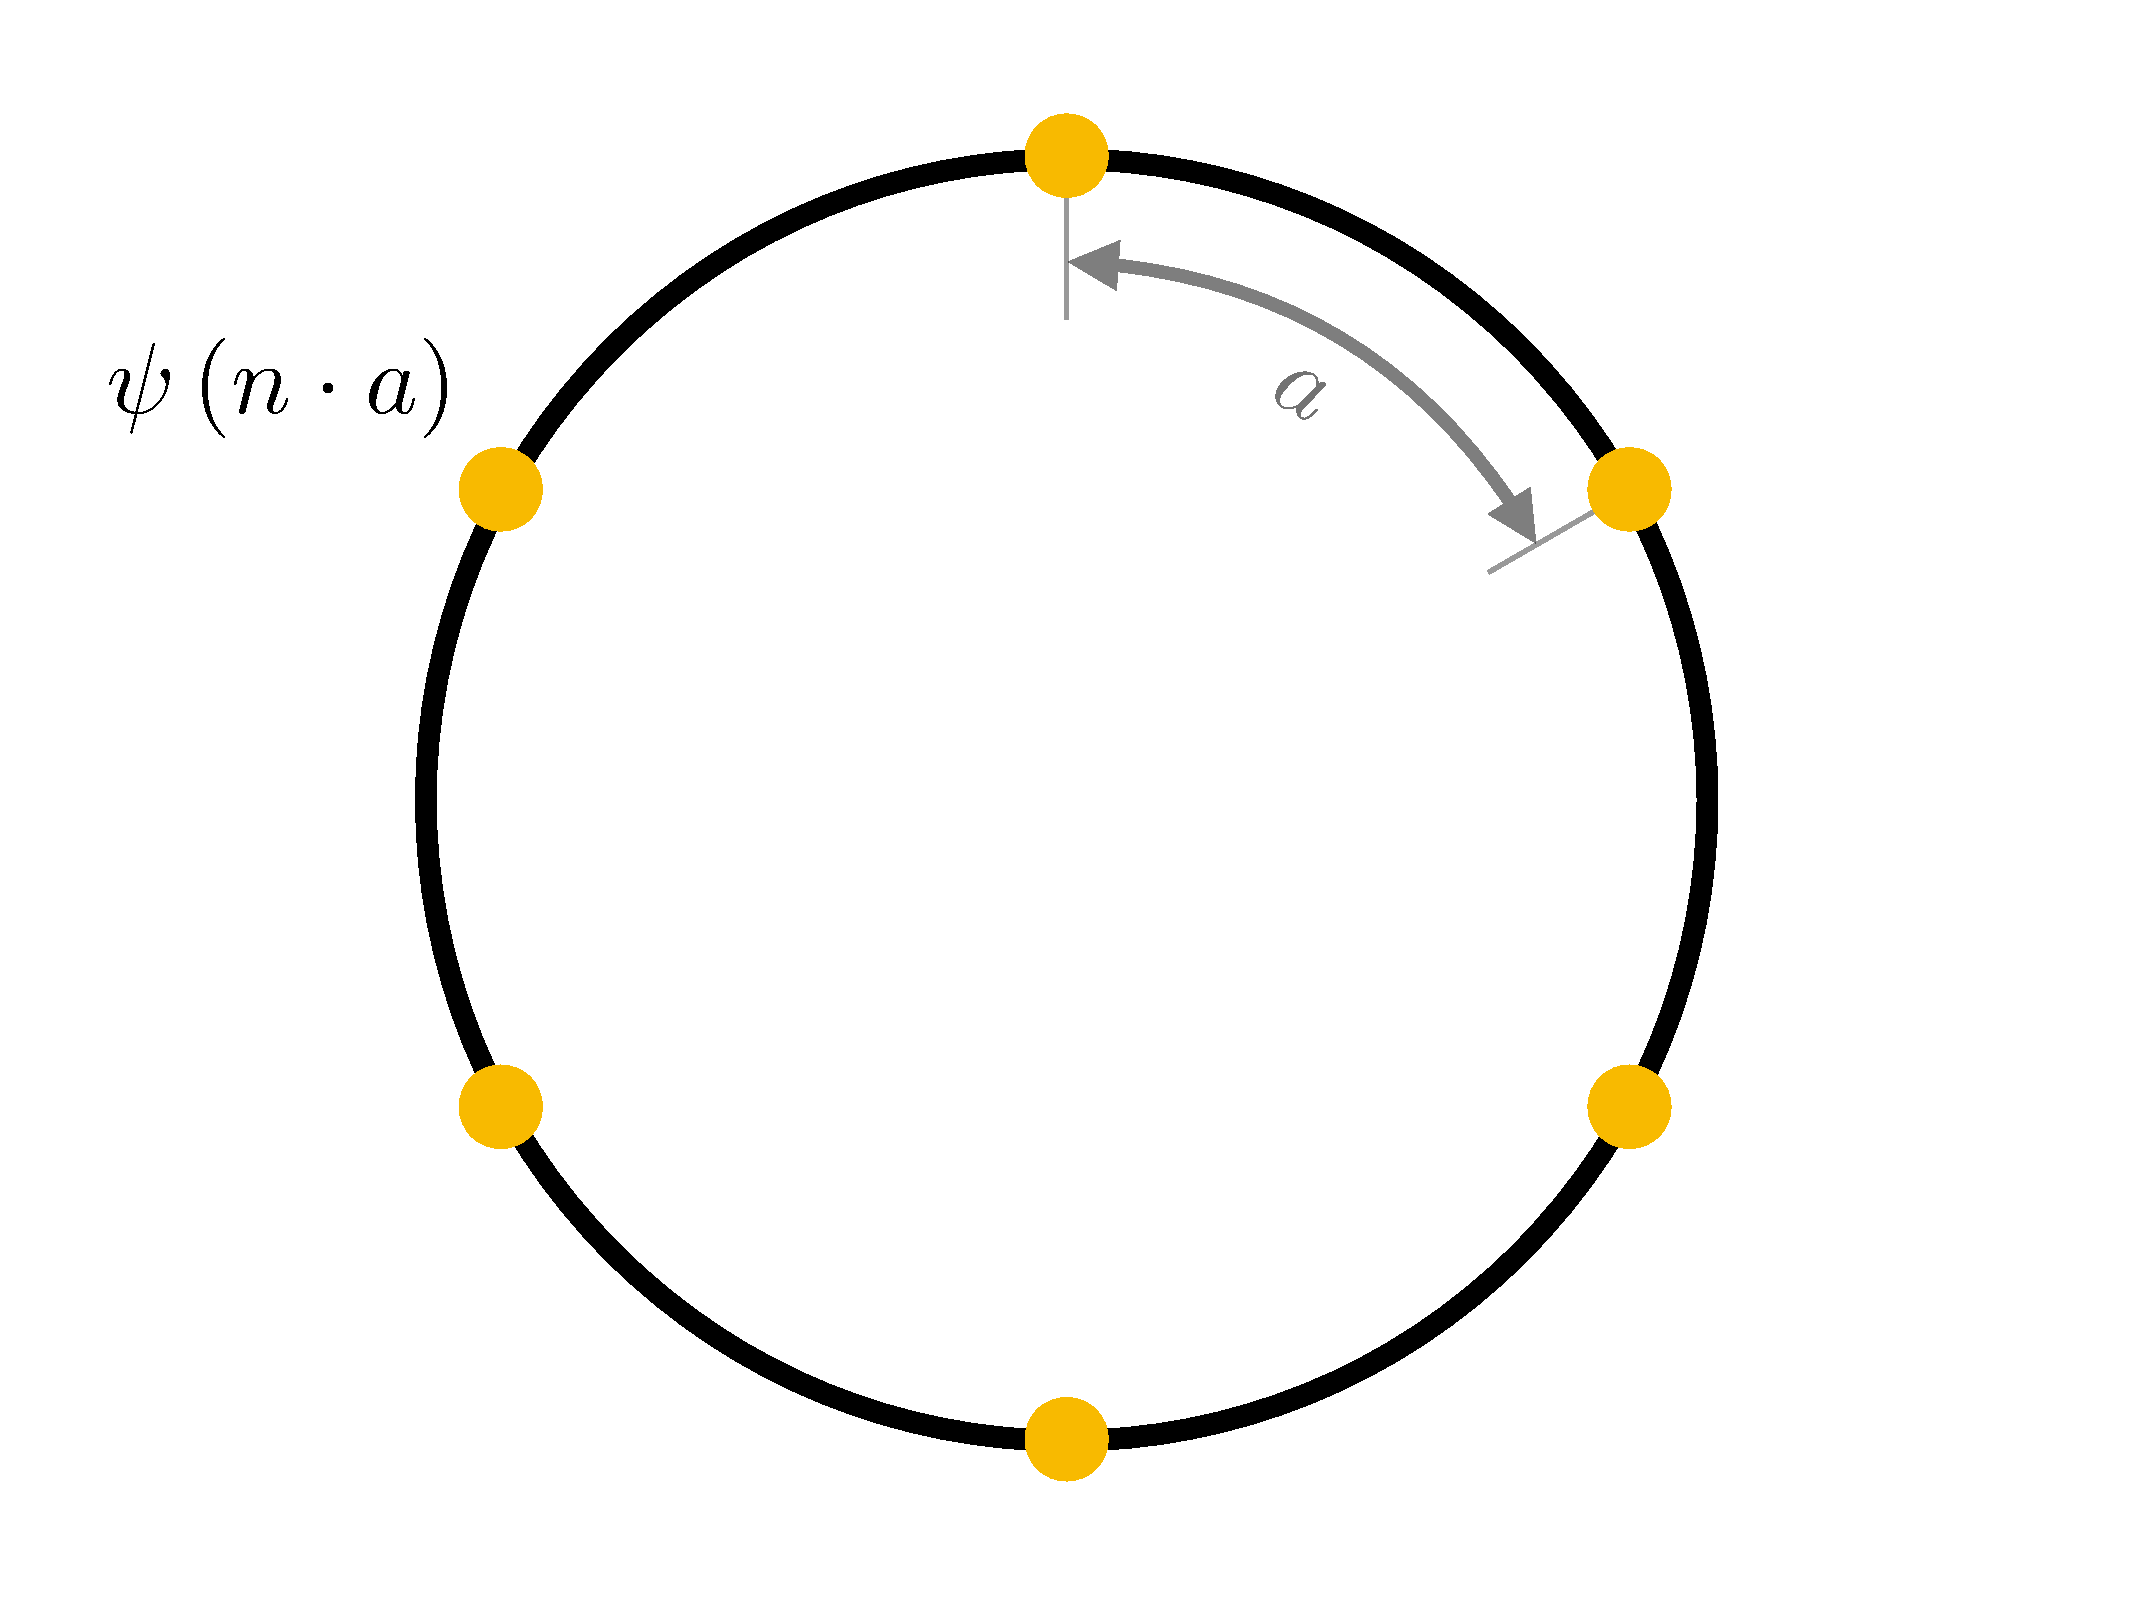
\includegraphics[width=\linewidth]{Figures/NJL1-model-solving/theoretical-fermion-lattice}
		\end{minipage}
	  \hspace{.025\linewidth}
		\begin{minipage}[c]{.45\linewidth}
			\centering
			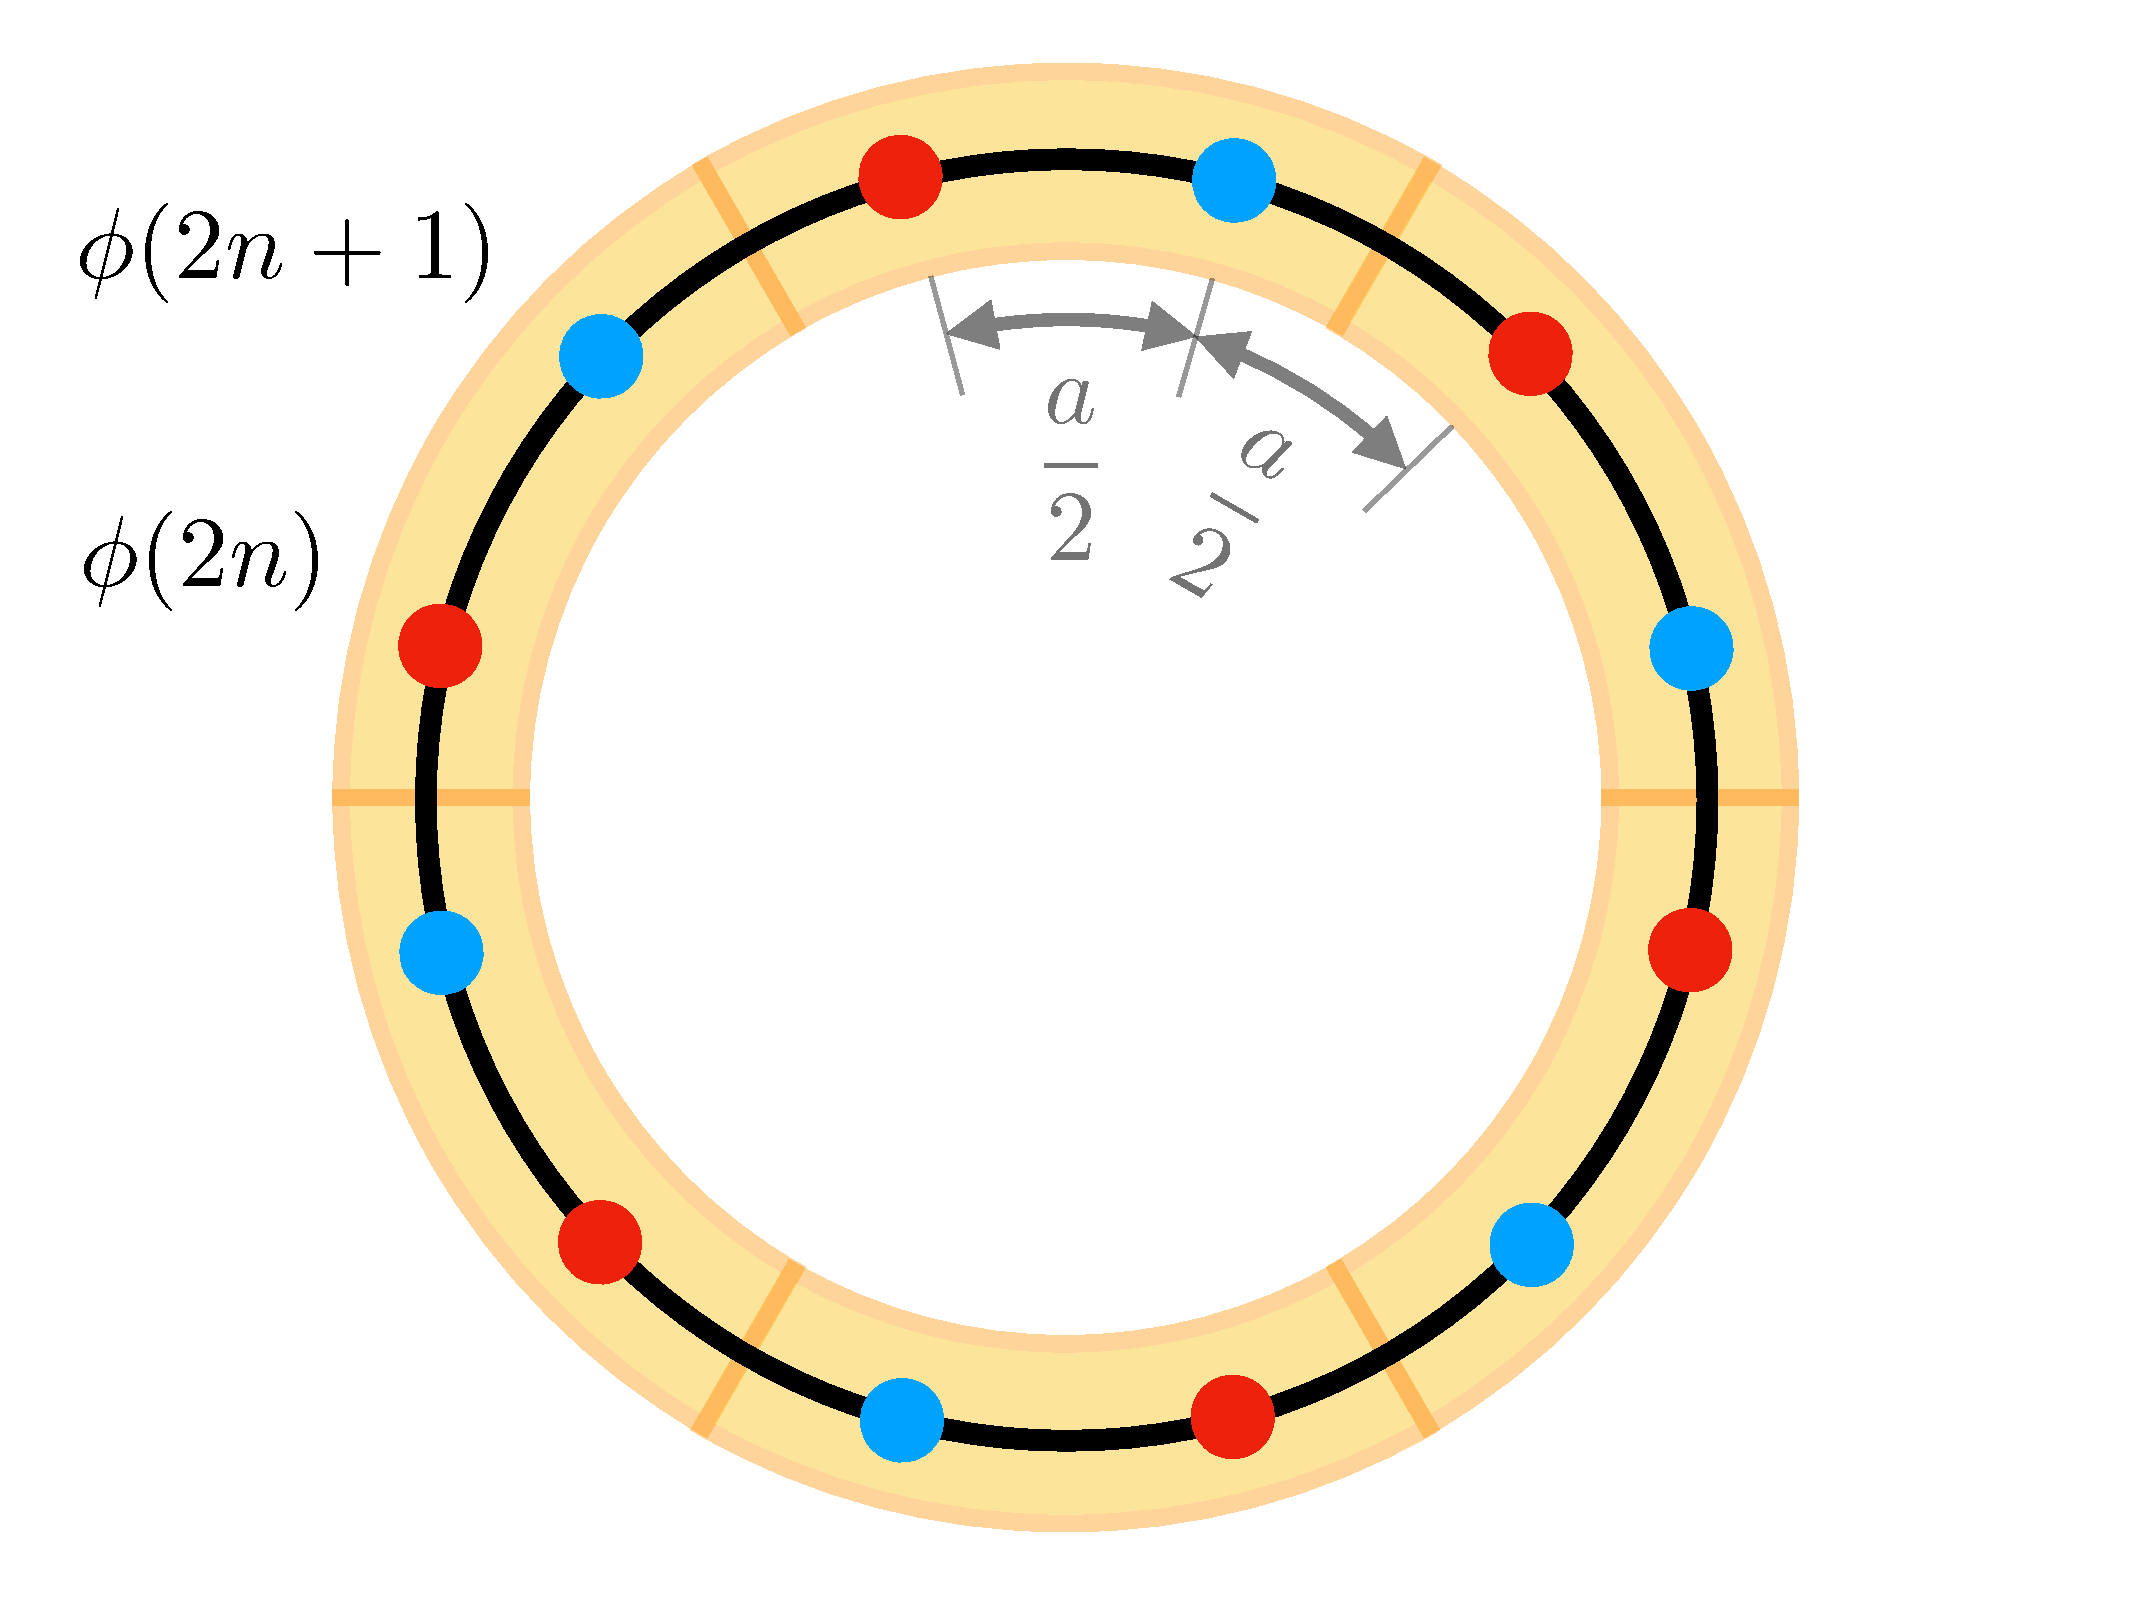
\includegraphics[width=\linewidth]{Figures/NJL1-model-solving/computational-fermion-lattice}
		\end{minipage}
		% \caption{Representations of a fermion lattice in $1+1$ dimensions, with periodic boundary conditions, and for $N=6$ theoretical lattice sites. (Left) Theoretical lattice. (Right) Staggered computational lattice.}
	  % \label{fig:staggered-fermion-lattice}
	\end{figure}

\break

	Sites in the staggered computational lattice are labeled using a parameter $n \in \mathds{Z}$ such that all evaluations of $\psi$ are made at integer multiples of the distance $a$:

	\begin{gather*}
	  \phi(n) \defeq \sqrt{a}
	    \begin{cases}
	      \psi_{+}\qty(\frac{n}{2}a) \qc &2 \mid n \\
	      \psi_{-}\qty(\frac{n-1}{2}a) \qc &2 \nmid n
	    \end{cases}
	\end{gather*}

	These newly defined operators obey the \textbf{canonical commutation relations for fermions}:

	\begin{gather*} \label{eq:fermion-canonical-commutation-relations}
	  \acom{\phi^{\dagger}(p)}{\phi(q)} = \delta_{pq} \qc
	  \acom{\phi(p)}{\phi(q)} = 0
	\end{gather*}

	Finally, thanks to the periodic boundary conditions, we can write:

	\begin{gather*}
	  H_{N}^{(K)} =
	    \frac{i}{a} \sum_{n=0}^{2N-1} \qty[
	    \phi^{\dagger}(n)\phi(n+1) - \phi^{\dagger}(n+1)\phi(n)]
	\end{gather*}

\break

	From this Hamiltonian, we can now recover the \textbf{masless Dirac equation} in the continuum limit; which serves as proof of correctness:

	\begin{gather*}
	  \dot{\phi}(n) = i\com{H_{N}^{(K)}}{\phi(n)} = \frac{\phi(n+1)-\phi(n-1)}{a}
	\end{gather*}

	In terms of the original fields, this is:

	\begin{gather*}
	  \dot{\psi_{+}} = \frac{\Delta \psi_{-}}{\Delta x} \qc
	  \dot{\psi_{-}} = \frac{\Delta \psi_{+}}{\Delta x}
	\end{gather*}

	Lastly, taking the limit when $a \ra 0$:

	\begin{gather*}
	  \pderivative{t}\psi = \hat{\alpha_1}\pderivative{x}\psi \\
	  \hat{\alpha_1} \defeq \gamma_{0}\gamma_{1} = \gamma^{0}\gamma_{1}
	    = -\gamma^{0}\gamma^{1} = \mqty[0 & 1 \\ 1 & 0]
	\end{gather*}

\break

	And it is now straight forward to obtain all other components of the Hamiltonian from the expressions in the Hamiltonian density, which are written in terms of \textbf{Dirac bilinears}.

	\vspace{1em}

	\begin{gather*}
	  H_{N} = H_{N}^{(M)} + H_{N}^{(K)} + H_{N}^{(I)}
	    \label{eq:NJL1-staggered-discretization} \\
	  H_{N}^{(M)} =
	    m \sum_{n=0}^{2N-1} (-1)^{n}\phi^{\dagger}(n)\phi(n) \\
	  H_{N}^{(K)} =
	    \frac{i}{a} \sum_{n=0}^{2N-1} \qty[
	    \phi^{\dagger}(n)\phi(n+1) - \phi^{\dagger}(n+1)\phi(n)] \\
	  H_{N}^{(I)} =
	    - \frac{1}{2a} G_{\pi} \sum_{n=0}^{N-1} \qty[
	      \phi^{\dagger}(2n)\phi(2n) - \phi^{\dagger}(2n+1)\phi(2n+1)
	    ]^{2}
	\end{gather*}

\end{frame}

%% ----------------------------------------------------------------------------

\subsection{Fermion-qubit mapping}

\begin{frame}{Fermion-qubit mapping}

	Generally speaking, quantum computers cannot measure any given operator directly. Therefore, in order to simulate this or any other Hamiltonian in a quantum processor, one needs to efficiently map its component operators onto ones suitable for evaluation in such machines. The most commonly used of these sets are Pauli operators along with the identity: this is what we will use and refer to as the \textbf{Pauli set}.

	\medskip

	It turns out that, in one spatial dimension, spin-$\frac{1}{2}$ particles (i.e. qubits) behave much like fermions. This allows us to implement a mapping between one and the other. The \textbf{Jordan-Wigner transform} associates spin ``down'' and ``up'' with occupied and unoccupied fermion states (or vice versa). Particularly, we will choose:

	\begin{align*}
		\ket{\ua} \equiv \ket{0} &\qc
			\ket{\da} \equiv \ket{1} \\
    \ket{\da} \equiv \phi^{\dagger}\ket{0} &\qc
			\ket{\ua} \equiv \phi\ket{1} \\[5pt]
		\phi \ra \sigma^{+} &\qc \phi^{\dagger} \ra \sigma^{-}
	\end{align*}

\end{frame}

%% ----------------------------------------------------------------------------

\begin{frame}[allowframebreaks]{Jordan-Wigner transform}

	To prove that this is valid, we can define the following equivalences by drawing inspiration from raising and lowering operators in angular momentum theory:

	\begin{align*}
		\sigma^{1} &\equiv \phi^{\dagger} + \phi \\
		\sigma^{2} &\equiv i\qty(\phi^{\dagger} - \phi) \\
		\sigma^{3} &\equiv 1 - 2\phi^{\dagger}\phi
	\end{align*}

	Making use of the properties of fermion creation and annihilation operators, comprised within their canonical commutation relations, these can be shown to behave algebraically like \textbf{Pauli matrices}:

	\begin{align*}
	  \com{\sigma^{p}}{\sigma^{q}} &= 2i\epsilon_{pqr}\sigma^{r} \\
	  \acom{\sigma^{p}}{\sigma^{q}} &= 2\delta_{pq}
	\end{align*}

\break

	We can recover the usual spin raising and lowering hermitian conjugate operators:

	\begin{gather}
	  \sigma^{\pm} \defeq \frac{1}{2}\qty(\sigma^{1} \pm i\sigma^{2})
	\end{gather}

	All this allows us to use these spins as a basic model for fermions:

	\begin{gather} \label{eq:anticommutator-for-single-particle-jordan-wigner}
	  \acom{\phi}{\phi^{\dagger}} = 1 \qra \acom{\sigma^{+}}{\sigma^{-}} = 1
	\end{gather}

	Unfortunately, this only works for single-fermion representations, and needs to be modified once we introduced more than one particle; since independent spins commute, while independent fermions anticommute.

	\begin{gather*}
	  \com{\sigma^{+}(p)}{\sigma^{-}(q)} = \delta_{pq} \qc
	    \acom{\sigma^{+}(p)}{\sigma^{-}(q)} \neq \delta_{pq} \\
	  \com{\phi(p)}{\phi^{\dagger}(q)} \neq \delta_{pq} \qc
	    \acom{\phi(p)}{\phi^{\dagger}(q)} = \delta_{pq}
	\end{gather*}

\break

	A way to fix this issue is by defining $N(l)=\phi^{\dagger}(l)\phi(l)$ as the hermitian number operator for state $l$, and attaching a so called unitary \textbf{string operator} $S(n)$ to the fermion operators:

	\begin{gather*}
		\begin{split}
			S(n)\phi(n) &\ra \sigma^{+}(n) \\
			\phi^{\dagger}(n)S^{\dagger}(n) &\ra \sigma^{-}(n)
		\end{split} \\
		S(n) = \exp[ -i\pi \sum_{l<n} \qty[N(l)+s(l)] ]
	\end{gather*}

	\vspace{-0.5em}

	The $s(l)$ terms in the string operator are scalars associated to gauge transformations and do not add much to the transform. With this new mapping, Pauli matrices get redefined to:

	\begin{align*}
		\sigma^{1}(n) &\equiv
			\phi^{\dagger}(n)S^{\dagger}(n) + S(n)\phi(n) \\
		\sigma^{2}(n) &\equiv
			i\qty[\phi^{\dagger}(n)S^{\dagger}(n) - S(n)\phi(n)] \\
		\sigma^{3}(n) &\equiv
			1 - 2\phi^{\dagger}(n)\phi(n)
	\end{align*}

\break

	We now retrieve the correct statistics. Of course, we would like to express the string operator in terms of the Pauli set so that we can move it to the other side of the transformation. Fortunately, we can do so by expanding the number operators:

	\begin{gather*}
	  \exp[\pm i\pi \sum_{l<n} N(l)] =
		  \prod_{l<n}\exp[\pm i\pi \phi^{\dagger}(l)\phi(l)] =
		  \prod_{l<n}\qty[1-2\phi^{\dagger}(l)\phi(l)] =
		  \prod_{l<n}\sigma^3(l) \\
		S(n) = \prod_{l<n} e^{-i\pi s(l)} \sigma^3(l)
	\end{gather*}

	Finally, our \textbf{choice of gauge} will be such that $s(l) = s \in (-1,1]$ $\forall l$ and the string operator is hermitian for all values of $n$. All in all, this can be achieved by making $s=0$, which gives:

	\begin{gather*}
		\phi(n) \ra \qty[\prod_{l<n} \sigma^3(l)]\sigma^{+}(n) \qc
		\phi^{\dagger}(n) \ra \qty[\prod_{l<n} \sigma^3(l)]\sigma^{-}(n)
	\end{gather*}

\end{frame}

%% ----------------------------------------------------------------------------

\begin{frame}[allowframebreaks]{Refactoring the NJL Hamiltonian}

	Now that we have a way of converting from fermion to spin operators, we can apply it to the NJL Hamiltonian:

	\begin{align*}
	  H_{N}^{(M)} &\qra
	    \frac{m}{2} \sum_{n=0}^{2N-1} (-1)^{n+1}\sigma^{3}(n) \\
	  H_{N}^{(K)} &\qra
	    \frac{i}{a} \sum_{n=0}^{2N-1}
	    \qty[\sigma^{-}(n)\sigma^{+}(n+1) - \sigma^{-}(n+1)\sigma^{+}(n)] \\
	  H_{N}^{(I)} &\qra
	    \frac{G_{\pi}}{4a} \sum_{n=0}^{N-1} \qty[\sigma^{3}(2n)\sigma^{3}(2n+1) - N]
	\end{align*}

	We will only be interested in studying the \textbf{Chiral limit} (i.e. $m=0$), which justifies dropping the entire mass term. From the interaction Hamiltonian we will get an adiabatic modification term of the form $\frac{G_{\pi}N}{4a}$; this will also be dropped for the moment.

\break

	Hence, with periodic boundary conditions $\sigma^{p}(N)=\sigma^{p}(0)$ and expressed in quantum computing notation $\qty(\mathds{1}_{n},X_{n},Y_{n},Z_{n}) \equiv \sigma^{p}(n)$ for $p=\qty(0,1,2,3)$, our refactored Hamiltonian $P_{N} \defeq 2aH_{N}$ will adopt the form:

	\begin{gather} \label{eq:NJL1-refactored-hamiltonian}
	  P_{N} =
	    \sum_{n=0}^{2N-1} \qty[X_{n+1} Y_{n} - Y_{n+1} X_{n}] +
	      \frac{G_{\pi}}{2} \sum_{n=0}^{N-1} Z_{2n+1} Z_{2n}
	\end{gather}

	One important feature of this operator is that its size (i.e. number of terms) \textbf{grows polynomially} with the size of the system $N$. It is also interesting to notice that this operator can be expressed in a recursive layout:

	\begin{align*}
		P_{N+1} =& P_{N}
				- Y_{2N-1} X_{0} + X_{2N-1} Y_{0} + Y_{2N+1} X_{0} - X_{2N+1} Y_{0} \\
			&+ X_{2N} Y_{2N-1} - Y_{2N} X_{2N-1} + X_{2N+1} Y_{2N} - Y_{2N+1} X_{2N}
				+ \frac{G_{\pi}}{2} \qty(Z_{2N+1} Z_{2N})
	\end{align*}

\end{frame}


%% ----------------------------------------------------------------------------

\subsection{Space parametrization and state preparation}

\begin{frame}{Space parametrization and state preparation}

	Once we have ways of measuring our Hamiltonian, we need to be able to explore different quantum states; a process known as \textbf{state preparation}. This can be achieved by parametrizing the Hilbert/Fock space of states representing the system, and finding a way to prepare the corresponding quantum state in the processor given any combination of those parameters.

	\begin{multicols}{2}

		For this task we will be employing some of the IBM-Q quantum computers and simulators; accessible through the cloud via the \texttt{Qiskit} framework. Nevertheless, there is one major shortcoming: the dimension of the space at hand grows exponentially with the number of qubits $2N$ used in the representation of the system. This means that the parametrization will become too large to handle both in state of the art and forthcoming machines unless it is treated in a smart way.

		\columnbreak

		\begin{center}
			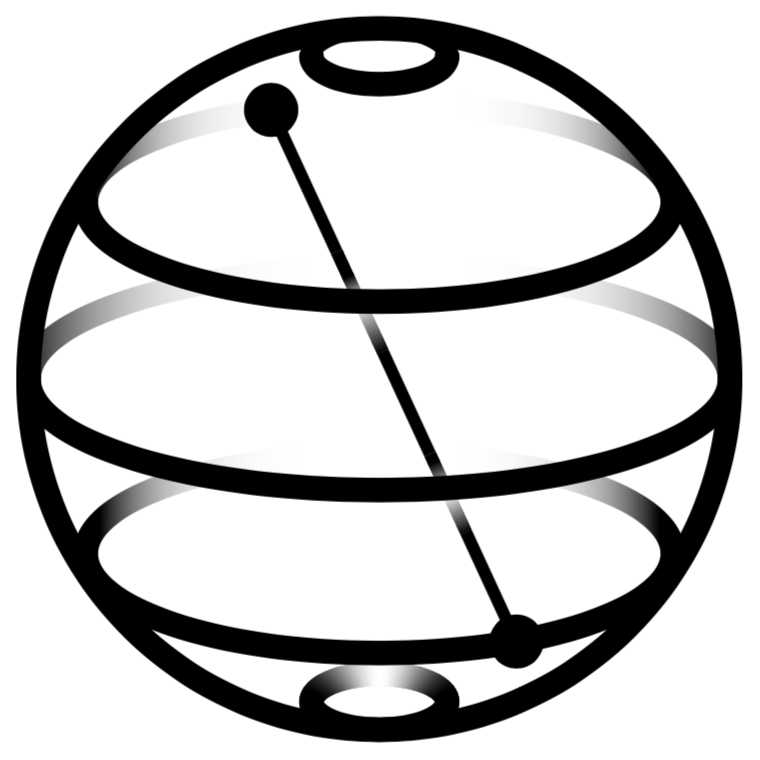
\includegraphics[width=.2\paperwidth]{Figures/qiskit}
		\end{center}
		\begin{center}
			
\includegraphics[width=.1\paperwidth]{Figures/ibm}
		\end{center}

	\end{multicols}

\end{frame}

%% ----------------------------------------------------------------------------

\begin{frame}[allowframebreaks]{Unitary coupled cluster}

	The motivation behind coupled cluster methods arises from the idea of explorinig only the regions of phase space close to an initial \textbf{reference state}. The choice of said reference state is of great importance for retreiving successful results. Let us begin by choosing the region of study in terms of \textbf{Hamming distance} (i.e. bit flips). This is sometimes called \textbf{configuration interaction} (CI). Using a notation where $\sigma^{p}_{n} \equiv \sigma^{p}(n)$ we can write any state one spin flip away from the initial reference state as:

	\begin{gather*}
	  \ket{\text{CI}_{1} \qty(z^{n})} \defeq
	    \sum_{n} z^{n} \sigma^{+}_{n} \ket{\text{SR}}
	\end{gather*}

	\vspace{-1em}

	This approach can be easily extended to account for more and more states:

	\begin{gather*}
	  \ket{\text{CI}_{k} \qty(\boldsymbol{z})} \defeq
	    \sum_{j=1}^{k} T_{j} \qty(z^{n_1,\cdots,n_j}) \ket{\text{SR}} \\
	  T_{j} \qty(z^{n_1,\cdots,n_j}) \defeq \sum_{n_1,\cdots,n_j}
	    z^{n_1,\cdots,n_j} \sigma^{+}_{n_1} \! \cdots \sigma^{+}_{n_j}
	\end{gather*}

\break

	However, this approach presents a number of deficiencies which render it non-optimal; the biggest one for us being that it presents no clear advatadge over classical state preparation. The idea behind \textbf{coupled cluster} (CC) consists on using the spin flips as generators instead:

	\begin{gather*}
	  \ket{\text{CC}_{k} \qty(\boldsymbol{z})} \defeq
	    \exp[\sum_{j=1}^{k} T_{j} \qty(z^{n_1,\cdots,n_j})]
	    \ket{\text{SR}}
	\end{gather*}

	In order to make this ansatz suitable for quantum processors, we need to express it in terms of unitary transformations. We have finally arrived at \textbf{unitary coupled cluster} (UCC):

	\begin{gather*}
	  \ket{\text{UCC}_{k} \qty(\boldsymbol{\theta},\boldsymbol{\eta})} \defeq
	    \exp[
	      \sum_{j=1}^{k} T_{j}^{-} \qty(\theta^{n_1,\cdots,n_j}) + i
	      \sum_{j=1}^{k} T_{j}^{+} \qty(\eta^{n_1,\cdots,n_j})
	    ]
	    \ket{\text{SR}} \\
	    T_{j}^{\pm} \qty(\theta^{n_1,\cdots,n_j}) \defeq
	      \sum_{n_1,\cdots,n_j} \theta^{n_1,\cdots,n_j} \qty(
	        \sigma^{+}_{n_1} \! \cdots \sigma^{+}_{n_j} \: \pm \:
	        \sigma^{-}_{n_1} \! \cdots \sigma^{-}_{n_j}
	      )
	\end{gather*}

\break

	Another important version of this ansatz is developed in a \textbf{fermionic basis} (i.e. for parametrizing Fock space instead of Hilbert space), and replaces spin-flips with changes in the state of particles. This is interesting because, due to the non-locality of the Jordan-Wigner transform, if we were to apply the unitary coupled cluster parametrization directly onto the Jorda-Wigner's mapping image (i.e. Hilbert space), we might be exploring uninteresting regions of the domain (i.e. Fock space) ---such as those containing symmetry-broken states. On top of that, this method is usually developed so that it \textbf{conserves the total number of particles} in the system; which is predefined through the fermion reference (FR):

	\begin{gather*}
	  \ket{\text{FUCC}_{k} \qty(\boldsymbol{\theta},\boldsymbol{\eta})} \defeq
	    \exp[
	      \sum_{j=1}^{k} F_{j}^{-} \qty(\theta^{p_1,\cdots,p_j,q_1\cdots,q_j}) +i
	      \sum_{j=1}^{k} F_{j}^{+} \qty(\eta^{p_1,\cdots,p_j,q_1\cdots,q_j})
	    ]
	    \ketf{\text{FR}}_{\mathcal{Q}} \\
	    F_{j}^{\pm} \qty(\theta^{p_1,\cdots,p_j,q_1\cdots,q_j}) \defeq
	      \sum_{\substack{q \in \mathcal{Q} \\ p \in \overline{\mathcal{Q}}}}
	      \theta^{p_1,\cdots,p_j,q_1\cdots,q_j} \qty(
	        \phi^{\dagger}_{p_1} \! \cdots \phi^{\dagger}_{p_j} \,
	        \phi_{q_1} \! \cdots \phi_{q_j} \: \pm \:
	        \phi^{\dagger}_{q_1} \! \cdots \phi^{\dagger}_{q_j} \,
	        \phi_{p_1} \! \cdots \phi_{p_j}
	      )
	\end{gather*}

\end{frame}

%% ----------------------------------------------------------------------------

\begin{frame}{Custom symmetry-based parametrization ansatz}

\end{frame}

%% ----------------------------------------------------------------------------

\begin{frame}{Parametrization ansatz implementation}

\end{frame}

%% ----------------------------------------------------------------------------

\subsection{Ground state energy}


%% ----------------------------------------------------------------------------
%% ----------------------------------------------------------------------------

\section{Conclusions and prospective work}


%% ----------------------------------------------------------------------------
%% BACK-MATTER
%% ----------------------------------------------------------------------------

\section{Bibliography}
%	\begin{frame}[allowframebreaks]{Bibliography}
\begin{frame}{Bibliography}

	\begin{thebibliography}{9}
		\setbeamertemplate{bibliography item}[online]
	\bibitem{hayden} \textbf{Hayden, P.} \emph{Quantum Computational Universe}
		\setbeamertemplate{bibliography item}[book]
	\bibitem{susskind_book} \textbf{Susskind, L. \& Friedman A.} \emph{Quantum Mechanics: The Theoretical Minimum}
		\setbeamertemplate{bibliography item}[book]
	\bibitem{nielsen} \textbf{Nielsen M.A. \& Chuang I.L.} \emph{Quantum Computation and Quantum Information}
		\setbeamertemplate{bibliography item}[article]
	\bibitem{ladd} \textbf{Lykken J.} \emph{Quantum Technologies for Quantum Science}
		\setbeamertemplate{bibliography item}[book]
	\bibitem{mermin} \textbf{Mermin N.D.} \emph{Quantum Computer Science: An Introduction}
		\setbeamertemplate{bibliography item}[article]
	\bibitem{ladd} \textbf{Ladd T.D. (et al.)} \emph{Quantum Computing}

	\end{thebibliography}

	\vspace{20pt}
	\begin{small}
	\begin{center}{
	\color{gray}
		\emph{"The only thing demonstrated by an impossibility proof is a lack of imagination."} \\
		\textbf{– John Stewart Bell –} }
	\end{center}
	\end{small}
\end{frame}

\FinalFrame

\end{document}
